\documentclass[aspectratio=169]{beamer}
\usepackage{mathpazo}
\usepackage{hyperref}
\usepackage{multimedia}
\usepackage{tcolorbox}
\usepackage{tabularx, colortbl}
\usepackage{appendixnumberbeamer}
\usepackage{tikz}
\usepackage{subcaption}
\usetikzlibrary{shadows}
\usepackage{booktabs,longtable}
\usepackage{tabularx}
\usepackage{graphicx}
\usetheme{default}
\usecolortheme{default}
\setbeamertemplate{itemize item}{%
    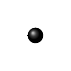
\begin{tikzpicture}
        \shade[ball color=black!100!yellow, preaction={fill=black,
opacity=.00,transform canvas={xshift=1mm,yshift=-1mm, yscale=0.5}}] (0,0) circle (0.6ex);
    \end{tikzpicture}
}
\setbeamertemplate{itemize subitem}{%
    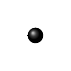
\begin{tikzpicture}
        \shade[ball color=black!100!white, preaction={fill=black,
        opacity=.00,transform canvas={xshift=1mm,yshift=-1mm, yscale=0.5}}] (0,0) circle (0.6ex);
    \end{tikzpicture}
}
\setbeamercolor{frametitle}{bg=white}
\setbeamercolor{frametitle}{fg=blue}
\setbeamercolor{background canvas}{bg=white}
\setbeamercolor{block body}{bg=mDarkTeal!30}
\setbeamercolor{block title}{bg=mDarkTeal,fg=black!2}
\setbeamertemplate{navigation symbols}{}
\setbeamercolor{background canvas}{bg=white}
% \setbeamertemplate{footline}[page number]
\newenvironment{stepenumerate}{\begin{enumerate}[<+->]}{\end{enumerate}}
\newenvironment{stepitemize}{\begin{itemize}[<+->]}{\end{itemize} }
\newenvironment{stepenumeratewithalert}{\begin{enumerate}[<+-| alert@+>]}{\end{enumerate}}
\newenvironment{stepitemizewithalert}{\begin{itemize}[<+-| alert@+>]}{\end{itemize} }

\title{\color{blue}
{\huge What Happens to Workers at Firms that Automate?}}
\author{
James Bessen, \textit{Boston University} \\
Maarten Goos, \textit{Utrecht University \& Instituut Gak} \\
Anna Salomons, \textit{Utrecht University \& Instituut Gak} \\
Wiljan van den Berge, \textit{Utrecht University \& CPB} \\
\\
}

% {\huge So-So Automation in Distorted Labor Markets}}
\date{forthcoming in Review of Economics and Statistics}

\begin{document}

{
% \pgfdeclareimage[height=\paperheight, width=\paperwidth]{myimage}{figures/selfcheckout.pdf}
% \usebackgroundtemplate{\tikz\node[opacity=0.3] {\pgfuseimage{myimage}};}
% \usebackgroundtemplate{\includegraphics[width=\paperwidth]{figures/background.png}}
\begin{frame}
\maketitle
\begin{tikzpicture}[overlay, remember picture]
\node[anchor= south west, xshift=7cm] at (current page.south west) {
\includegraphics[width=1cm]{figures/uu.png}};
\end{tikzpicture}
\begin{tikzpicture}[overlay, remember picture]
\node[anchor= south west, xshift=9cm] at (current page.south west) {
\includegraphics[width=1cm]{figures/gak.jpeg}};
\end{tikzpicture}
\end{frame}
}

\AtBeginSection[]
{
\begin{frame}{Outline}
    \tableofcontents[currentsection]
\end{frame}
}

\begin{frame}
\frametitle{Does automation threaten work?}
\begin{columns}
\begin{column}{0.5\textwidth}  %%<--- here
    \begin{center}
     \includegraphics[width=0.5\textwidth]{Paper-Revisions/graphics/Joost-Swarte-Robot-Shadow.pdf}
     \end{center}
\end{column}
\begin{column}{0.5\textwidth}
   \begin{itemize}
       \item<1-> Task-based theories of \textbf{automation as labor-replacing technology} \textcolor{gray}{\scriptsize{Autor\&al.(03), Acemoglu\&Autor(11), Acemoglu\&Restrepo(18,22)}}\medskip
       \item<2-> Different from previous work assuming \textbf{Harrod-, Solow-, or Hicks-neutral} tech progress \textcolor{gray}{\scriptsize{Uzawa(61), Katz\&Murphy(92), Piketty(14), Krusell\&al.(00)}}\medskip
       \item<3-> Models of automation more easily predict decreases in labor share and labor demand \textcolor{gray}{\scriptsize{Restrepo(23), Grossman\&Oberfield(22)}}
   \end{itemize}
\end{column}
\end{columns}
\end{frame}

\begin{frame}{Automation and labor markets: emerging evidence \hyperlink{otherstudies}{\beamerbutton{overview}}} \label{literature}
\begin{itemize}
  \item<1-> \textbf{Macro-level evidence} on aggregate changes in occupations, sectors, labor share, wage inequality \textcolor{gray}{\scriptsize{Acemoglu\&Restrepo(20,22), Boustan\&al.(22), Hubmer\&Restrepo(21), Autor\&al.(20)}}\medskip
  \item<2-> \textbf{Micro-level evidence} on firm-level adoption of robots in manufacturing on firm-level outcomes \textcolor{gray}{\scriptsize{Aghion\&al.(23), Bonfiglioli\&etal.(22), Humlum(21), Hirvonen\&etal.(22)}}\medskip
  \item<3-> Challenges for micro-level evidence of automation on labor demand: \medskip
  \begin{itemize}
  \item measures of \textbf{automation beyond robotics} \medskip
  \item \textbf{worker-level} adjustments \medskip
  \item \textbf{credible research design} given larger firms invest more in automation
  \end{itemize}
\end{itemize} 
\end{frame}

\begin{frame}{Contributions}
\begin{enumerate}
    \item<1-> Measure of \textbf{firm-level automation expenditures} across sectors \bigskip
    \item<2-> Examine \textbf{worker-level impacts} of automation \bigskip
    \item<3-> \textbf{Event-study DiD design} leveraging the timing of automation events
    \bigskip %% We develop a model to show the assumptions required for this to work.
    \item<4-> Compare impacts of \textbf{automation versus computerization}\bigskip
    \item<5-> Ideas for examining \textbf{role of worker power}
\end{enumerate}
\end{frame}

%%%%%%%%%%%%%%%%%%%%%%%%%%%%%%%%%%%%%%%%%%%%%%%%%%%%%%%%%%%%%%%%%%%%%%
\section{Data}
%%%%%%%%%%%%%%%%%%%%%%%%%%%%%%%%%%%%%%%%%%%%%%%%%%%%%%%%%%%%%%%%%%%%%%

\begin{frame}{Data from Statistics Netherlands %\hyperlink{data_cleaning}{\beamergotobutton{Data cleaning}}
} \label{data}
\begin{itemize}
\item<1-> Annual \textbf{survey of private non-financial firms}, incl. \textbf{automation costs}:  \medskip
	\begin{itemize}
	\item Described as ``expenditures on third-party automation services'' \medskip
	\item Automation expenditures are an official book-keeping entry $\Rightarrow$ well measured \medskip
        \item Pervasive across time, sectors and firm sizes \medskip
        \item Correlated with process innovation and automation technologies \hyperlink{autom_innovation}{\beamerbutton{more}} \medskip
        \item Correlated with automation imports \hyperlink{sumstat_imports_sector}{\beamerbutton{more}} \medskip
	\end{itemize}
\item<2-> Administrative daily \textbf{matched employer-employee records} \hyperlink{data_cleaning}{\beamerbutton{more}} \medskip
\item<2-> Years \textbf{2000-2016} \medskip
\end{itemize} \medskip
\end{frame}

\begin{frame}{Automation costs per worker over time \hyperlink{des_autom}{\beamerbutton{more}}} \label{des_autom_time} 
\noindent \begin{center}
	\includegraphics[height=0.8\paperheight]{Paper-Revisions/graphics/des_autom_pw_overtime.PDF}
	\end{center}
\footnotesize
\end{frame}

\begin{frame}{Automation occurs in all sectors} \label{des_autom_sector}
\footnotesize
	\noindent 
        \begin{table}[t!]
	  \centering
	    \begin{threeparttable}
	    \scalebox{0.9}{
            \begin{tabular}{lcccccccc}
	    \toprule
	    \addlinespace  
	          & \multicolumn{2}{c}{\textbf{Mean cost level}} &       & \multicolumn{2}{c}{\textbf{Cost share (\%)}} &       & \multicolumn{2}{c}{\textbf{Nr of obs}} \\
	    \textbf{Sector} & Total & Per worker &       & \textit{Mean} & \textit{SD} &       & \textit{Firms} & \textit{Firms $\times$ yrs} \\
	    \midrule
	    Manufacturing & 430,091 & 1,076 &       & 0.36  & 0.58  &       & 5,522 & 44,393 \\
	    Construction & 78,128 & 451   &       & 0.20  & 0.36  &       & 4,429 & 28,200 \\
	    Wholesale \& retail trade & 116,308 & 1,177 &       & 0.31  & 0.80  &       & 10,903 & 75,135 \\
	    Transportation \& storage & 279,324 & 907   &       & 0.41  & 1.06  &       & 3,125 & 21,268 \\
	    Accommodation \& food serving & 55,714 & 245   &       & 0.30  & 0.50  &       & 1,182 & 6,535 \\
	    Information \& communication & 444,364 & 1,789 &       & 0.85  & 2.92  &       & 2,646 & 16,929 \\
	    Prof'l, scientific, \& technical activities & 150,766 & 1,285 &       & 1.02  & 1.75  &       & 3,935 & 23,367 \\
	    Administrative \& support activities & 133,437 & 839   &       & 0.50  & 1.19  &       & 3,825 & 22,796 \\
	    \bottomrule
	    \end{tabular}}
                \begin{tablenotes}
			\footnotesize
	         	 \item \emph{Notes:} Automation cost level in 2015 euros, automation cost shares as a percentage of total costs, excluding automation costs. Total firms is N=35,567; Total firms $\times$ years is 238,623. 
	           \end{tablenotes}
	          \end{threeparttable}
 \end{table}
\begin{itemize}  
\end{itemize}	
\end{frame}

\begin{frame}{Automation costs by firm size} \label{des_autom_size}
\footnotesize
	\noindent
	\begin{table}[t!]
	     \begin{threeparttable}
            \scalebox{0.9}{
	    \begin{tabular}{lcccccccccc}
	    \toprule
	          & \multicolumn{1}{l}{\textbf{Total cost}} &       & \multicolumn{2}{c}{\textbf{Cost per worker}} &       & \multicolumn{2}{c}{\textbf{Cost share (\%)}} &       & \multicolumn{2}{c}{\textbf{Nr of obs}} \\
	    \textbf{Firm size class} & Mean  &       & Mean  & SD    &       & Mean  & SD    &       & \textit{Firms} & \textit{Firms $\times$ yrs} \\
	    \midrule
	    1-19 employees & 12,270 &       & 921   & 14,571 &       & 0.4   & 1.3   &       & 9,495 & 48,052 \\
	    20-49 employees & 27,693 &       & 893   & 4,547 &       & 0.42  & 1.34  &       & 13,424 & 86,540 \\
	    50-99 employees & 61,460 &       & 953   & 4,345 &       & 0.42  & 0.96  &       & 6,186 & 47,038 \\
	    100-199 employees & 144,912 &       & 1,135 & 5,813 &       & 0.44  & 0.94  &       & 3,412 & 28,660 \\
	    200-499 employees & 406,534 &       & 1,574 & 21,314 &       & 0.51  & 1.11  &       & 1,941 & 17,852 \\
	    $\geq$500 employees & 3,161,867 &       & 2,124 & 14,294 &       & 0.76  & 1.6   &       & 1,109 & 10,481 \\
	    \bottomrule
	    \end{tabular}}
	    \begin{tablenotes}
			\footnotesize
	         	 \item \emph{Notes:} Automation cost level in 2015 euros, automation cost shares as a percentage of total costs, excluding automation costs. Total firms is N=35,567; Total firms $\times$ years is 238,623. 
	           \end{tablenotes}
	          \end{threeparttable}
	\end{table}
\end{frame}

%%%%%%%%%%%%%%%%%%%%%%%%%%%%%%%%%%%%%%%%%%%%%%%%%%%%%%%%%%%%%%%%%%%%%%
\section{Defining and explaining automation events}
%%%%%%%%%%%%%%%%%%%%%%%%%%%%%%%%%%%%%%%%%%%%%%%%%%%%%%%%%%%%%%%%%%%%%%

\begin{frame}{Defining spikes in automation cost shares} \label{spikes}
\noindent 
\begin{itemize}
\item Firms have \textbf{spikes in automation cost shares over time} \medskip 
\item Firm $j$ has an automation cost share spike in year  $\tau$ if:
\begin{equation*} 
spike_{j\tau} = \mathbb{1}\left\{ \frac{AC_{j\tau}}{\overline{TC}_{j}}\geq3\times \frac{1}{T-1} \sum_{t \neq \tau}^{T}\left(\frac{{AC}_{jt}}{\overline{TC}_{j}}\right)\right\}
\end{equation*}
%\item Keep spikes where automation cost share $>$ p25 of non-zero automation cost share distribution
%\medskip
%no mechanical correlation with firm characteristics
\item Of 35K firms, 10K have at least 1 spike, 8K have exactly 1 spike \hyperlink{spikefrequency}{\beamerbutton{more}} \medskip
\item A firm's \textbf{first spike is its automation event}
\end{itemize}
\end{frame}

\begin{frame}{Automation cost shares around automation events}
\centering
\includegraphics[height=0.45\paperwidth,keepaspectratio]{Paper-Revisions/graphics/des_mfgraph_autom.PDF}
%\hyperlink{des_spike_freq}{\beamerbutton{spike frequencies}}
%\hyperlink{why_spike}{\beamergotobutton{Lumpy investments}}
\end{frame}

\begin{frame}{A model to explain automation events \hyperlink{modelA}{\beamerbutton{model}}} \label{model} 
A model of monopolistic competition with endogenous firm-level automation: \medskip
\begin{itemize}
    \item \textbf{Automation}: task-based model in which $K$ directly substitutes for $L$ in tasks (ignoring other types of tech progress) \textcolor{gray}{\scriptsize{Acemoglu\&Restrepo(18,22)}} \medskip
    \item \textbf{Automation events}: automation is fixed and irreversible investment, spikes in automation cost shares within firms over time \textcolor{gray}{\scriptsize{Haltiwanger(99), Doms\&Dunne(98)}} \medskip
    \item \textbf{Product demand shocks} to explain why firms with automation events grow faster than firms without \textcolor{gray}{\scriptsize{Bonfiglioli\&al.(22)}}
\end{itemize}
\end{frame}

\frame{\frametitle{The firm's decision to automate} 
\begin{itemize}
\item<1-> If firm $j$ automates, \textbf{its output price decreases} to technology frontier:
    \begin{equation} 
P_{jt} =
\begin{cases}
P_{jt-1} \hspace{0.6cm} \text{ if }   D_{jt-1} = 0 \\ 
\mathcal{P}_{t} \hspace{1cm} \text{ if }   D_{jt-1} = 1 \text{ with } \mathcal{P}_{t} = \mu \mathcal{P}_{t-1} \text{ with } \mu < 1
\end{cases} \nonumber
\end{equation}
\item<2-> Firm $j$ chooses $D_{j0},D_{j1},... $ to \textbf{maximize expected net profits}:
    \begin{equation}
\max_{D_{j0},D_{j1},...} \mathbb{E} \sum_{t=0}^{\infty} \beta^{t} \left[ \sigma^{-1}Y_{t} \epsilon_{jt}^{\sigma-1} \left[ \frac{P_{jt}}{\mathcal{P}_{t}}\right] ^{(1 - \sigma)} - D_{jt} F_{jt} \right]  \nonumber
\end{equation}
with $F_{jt}$ the cost of automation incl. employment adjustment \medskip
\item<3-> $F_{jt}$ is fixed and irreversible s.t. \textbf{spikes in automation cost shares} over time
\end{itemize}
}

\begin{frame}{The impact of automation events on labor demand} 
\begin{itemize}
\item<1-> \textbf{Unconditional labor demand} is given by:
    \begin{equation} \nonumber
    L_{jt} = \left[ \frac{\sigma -1}{\sigma} \right]^{\sigma} Y_{t} \epsilon_{jt}^{\sigma-1} W_{t}^{- \sigma} \textcolor{orange}{[1-I_{jt}]} \textcolor{blue}{\left[ \left[ \frac{W_{t}}{R_{t}} \right]^{I_{jt}} \Psi_{H}(I_{jt}) \right]^{\sigma -1}}
\end{equation} 
with $I_{jt} \in [0,1]$ share of tasks that are automated \medskip
\item<1-> In $t-1$, the firm chooses $I_{jt}=I_{jt-1}$ or $I_{jt}=\mathcal{I}_{t}$ which increases over time \medskip
\item<1-> Increase in $ I_{jt}$ reduces labor demand if \textcolor{orange}{displacement effect} $>$ \textcolor{blue}{productivity effect} \medskip
\item<2-> \textbf{Product demand shock} affects both labor demand and automation
\end{itemize}
\end{frame}

\begin{frame}{Ever-automators have faster employment growth than never-automators}
\centering
\includegraphics[height=0.45\paperwidth,keepaspectratio]{Paper-Revisions/graphics/des_firm_emp_scaled.pdf}
%\hyperlink{des_spike_freq}{\beamerbutton{spike frequencies}}
%\hyperlink{why_spike}{\beamergotobutton{Lumpy investments}}
\end{frame}

\begin{frame}{Identifying assumptions for an event-study DiD design}
    \begin{enumerate}
        \item<1-> \textbf{Parallel trends in post-treatment periods}: \medskip
        \begin{itemize}
            \item Average outcomes for treated would change same as for controls if no treatment \medskip
            \item Not true when comparing ever-automating with never-automating firms \medskip
            \item Only use firms with automation events and exploit event timing not incidence \medskip
        \end{itemize}
        \item<2-> \textbf{No anticipation in pre-treatment periods}: \medskip
        \begin{itemize}
            \item Average outcomes for treated same if no treatment \medskip
            \item Firms do not invest in automation before an automation event \medskip
            \item Focus on incumbent workers employed at their firm 3 yrs prior automation
        \end{itemize}
    \end{enumerate}
\end{frame}

%%%%%%%%%%%%%%%%%%%%%%%%%%%%%%%%%%%%%%%%%%%%%%%%%%%%%%%%%%%%%%%%%%%%%%
\section{Stacked DiD estimates of worker-level impacts}
%%%%%%%%%%%%%%%%%%%%%%%%%%%%%%%%%%%%%%%%%%%%%%%%%%%%%%%%%%%%%%%%%%%%%%

\begin{frame}{Stacking the data}
    \begin{itemize}
    \item<1-> Consider event window of 3 yrs before and 5 yrs after \medskip
    \item<1-> For each year $ 2003 \leq t \leq 2011 $, create 9 \textbf{group-specific data sets} of workers treated in $t$ and control workers treated at least 5 yrs later \medskip
    \item<2-> We have excluded forbidden comparisons \textcolor{gray}{\scriptsize{Borusyak\&al.(23), Goodman-Bacon(21)}} \hyperlink{forbidden}{\beamerbutton{more}}  \medskip
    \item<3-> Stack 9 group-specific data sets into a single \textbf{stacked data set} \medskip
    \item<4-> Do this for incumbent workers (with $ \geqslant $ 3 yrs of tenure at their firm in year $t-1$)
    \end{itemize}
\end{frame}

\begin{frame}{TWFE event-study DiD specification using stacked data}
\begin{itemize}
\item<1-> Using stacked data, regress standard TWFE event-study DiD specification:
\begin{equation} \label{eq_stackedDiD}
Y_{i,j,t} = \alpha_{i} + \alpha_{t} + \sum_{e=-3}^{-2}\gamma_{e}^{PRE} D_{e} \times D_{i} + \sum_{e=0}^{4}\gamma_{e}^{POST} D_{e} \times D_{i} + \lambda X_{i,j,t} + \varepsilon_{i,j,t} \nonumber
\end{equation}
\item[]<1-> with $ \alpha_{i}$ individual-group FE and $ \alpha_{t}$ calendar year-group FE \medskip
\item<2-> $\hat{\gamma}_{e}$ is a variance-weighted average of group-specific $ATT$s \hyperlink{otherest}{\beamerbutton{alternatives}} \medskip
\item<3-> $X$ includes age, age squared (with time-invariant char. absorbed by $ \alpha_{i}$) \medskip
\item<3-> S.e. are clustered at the treatment-level (i.e. all workers at a firm in $t-1$)
\end{itemize}
\end{frame}

\begin{frame}{Loss in annual earnings totals 10\% of one annual wage after 5 yrs} 
\noindent \begin{center}
	\includegraphics[width=0.65\paperwidth]{Paper-Revisions/graphics/w_relwage_inc_k5_d7.PDF}
    %\item \footnotesize{323 euros lost in treatment year, 3,839 euros after 5 years in total}
   % \item \footnotesize{\hyperlink{other}{\beamergotobutton{Heterogeneity and additional results}} }
   	\end{center}
\end{frame}
%1 euro invested per worker leads to a loss of around 0.30 euros of per incumbent worker in the automation year, and 2 euros after 5 years

\begin{frame}{Hazard of leaving the firm increases by a total of 6.5ppt after 5 yrs} \label{leave}
\noindent \begin{center}
	\includegraphics[width=0.65\paperwidth]{Paper-Revisions/graphics/w_leave_inc_k5_d7.PDF}
%		\begin{tablenotes}
  %  \item \footnotesize{Hazard rates for CG incumbents are 9.6\% in t=0 and 8.8\% in t=4 (40\%$\uparrow$)}
 %   \end{tablenotes}
	\end{center}
\end{frame}

\begin{frame}{Annual days in non-emp. increase by a total of 18 days after 5 yrs} \label{nonemp}
\noindent \begin{center}
	\includegraphics[width=0.65\paperwidth]{Paper-Revisions/graphics/w_nonemp_inc_k5_d7.PDF}
%	\begin{tablenotes}
 %          \item \footnotesize{Annual non-employment days for CG incumbents are 5.7 in t=0 and 28 in t=4 (20\%$\uparrow$)}
 %   \end{tablenotes}
	\end{center}
\end{frame}

\begin{frame}{Annual income from unemployment benefits increases} \label{benefits_split}
\noindent \begin{center}
	\includegraphics[width=0.75\textwidth]{Paper-Revisions/graphics/w_benefits_inc_k5_d7.PDF}
		\end{center}
\end{frame}

\begin{frame}{Probability of early retirement increases by a total of 2.5ppt after 5 yrs}
\noindent \begin{center}
	\includegraphics[width=0.75\textwidth]{Paper-Revisions/graphics/w_retire_inc_k5_d7.PDF}
    \end{center}
\end{frame}

\begin{frame}{A summary of findings}
\noindent \begin{center}
	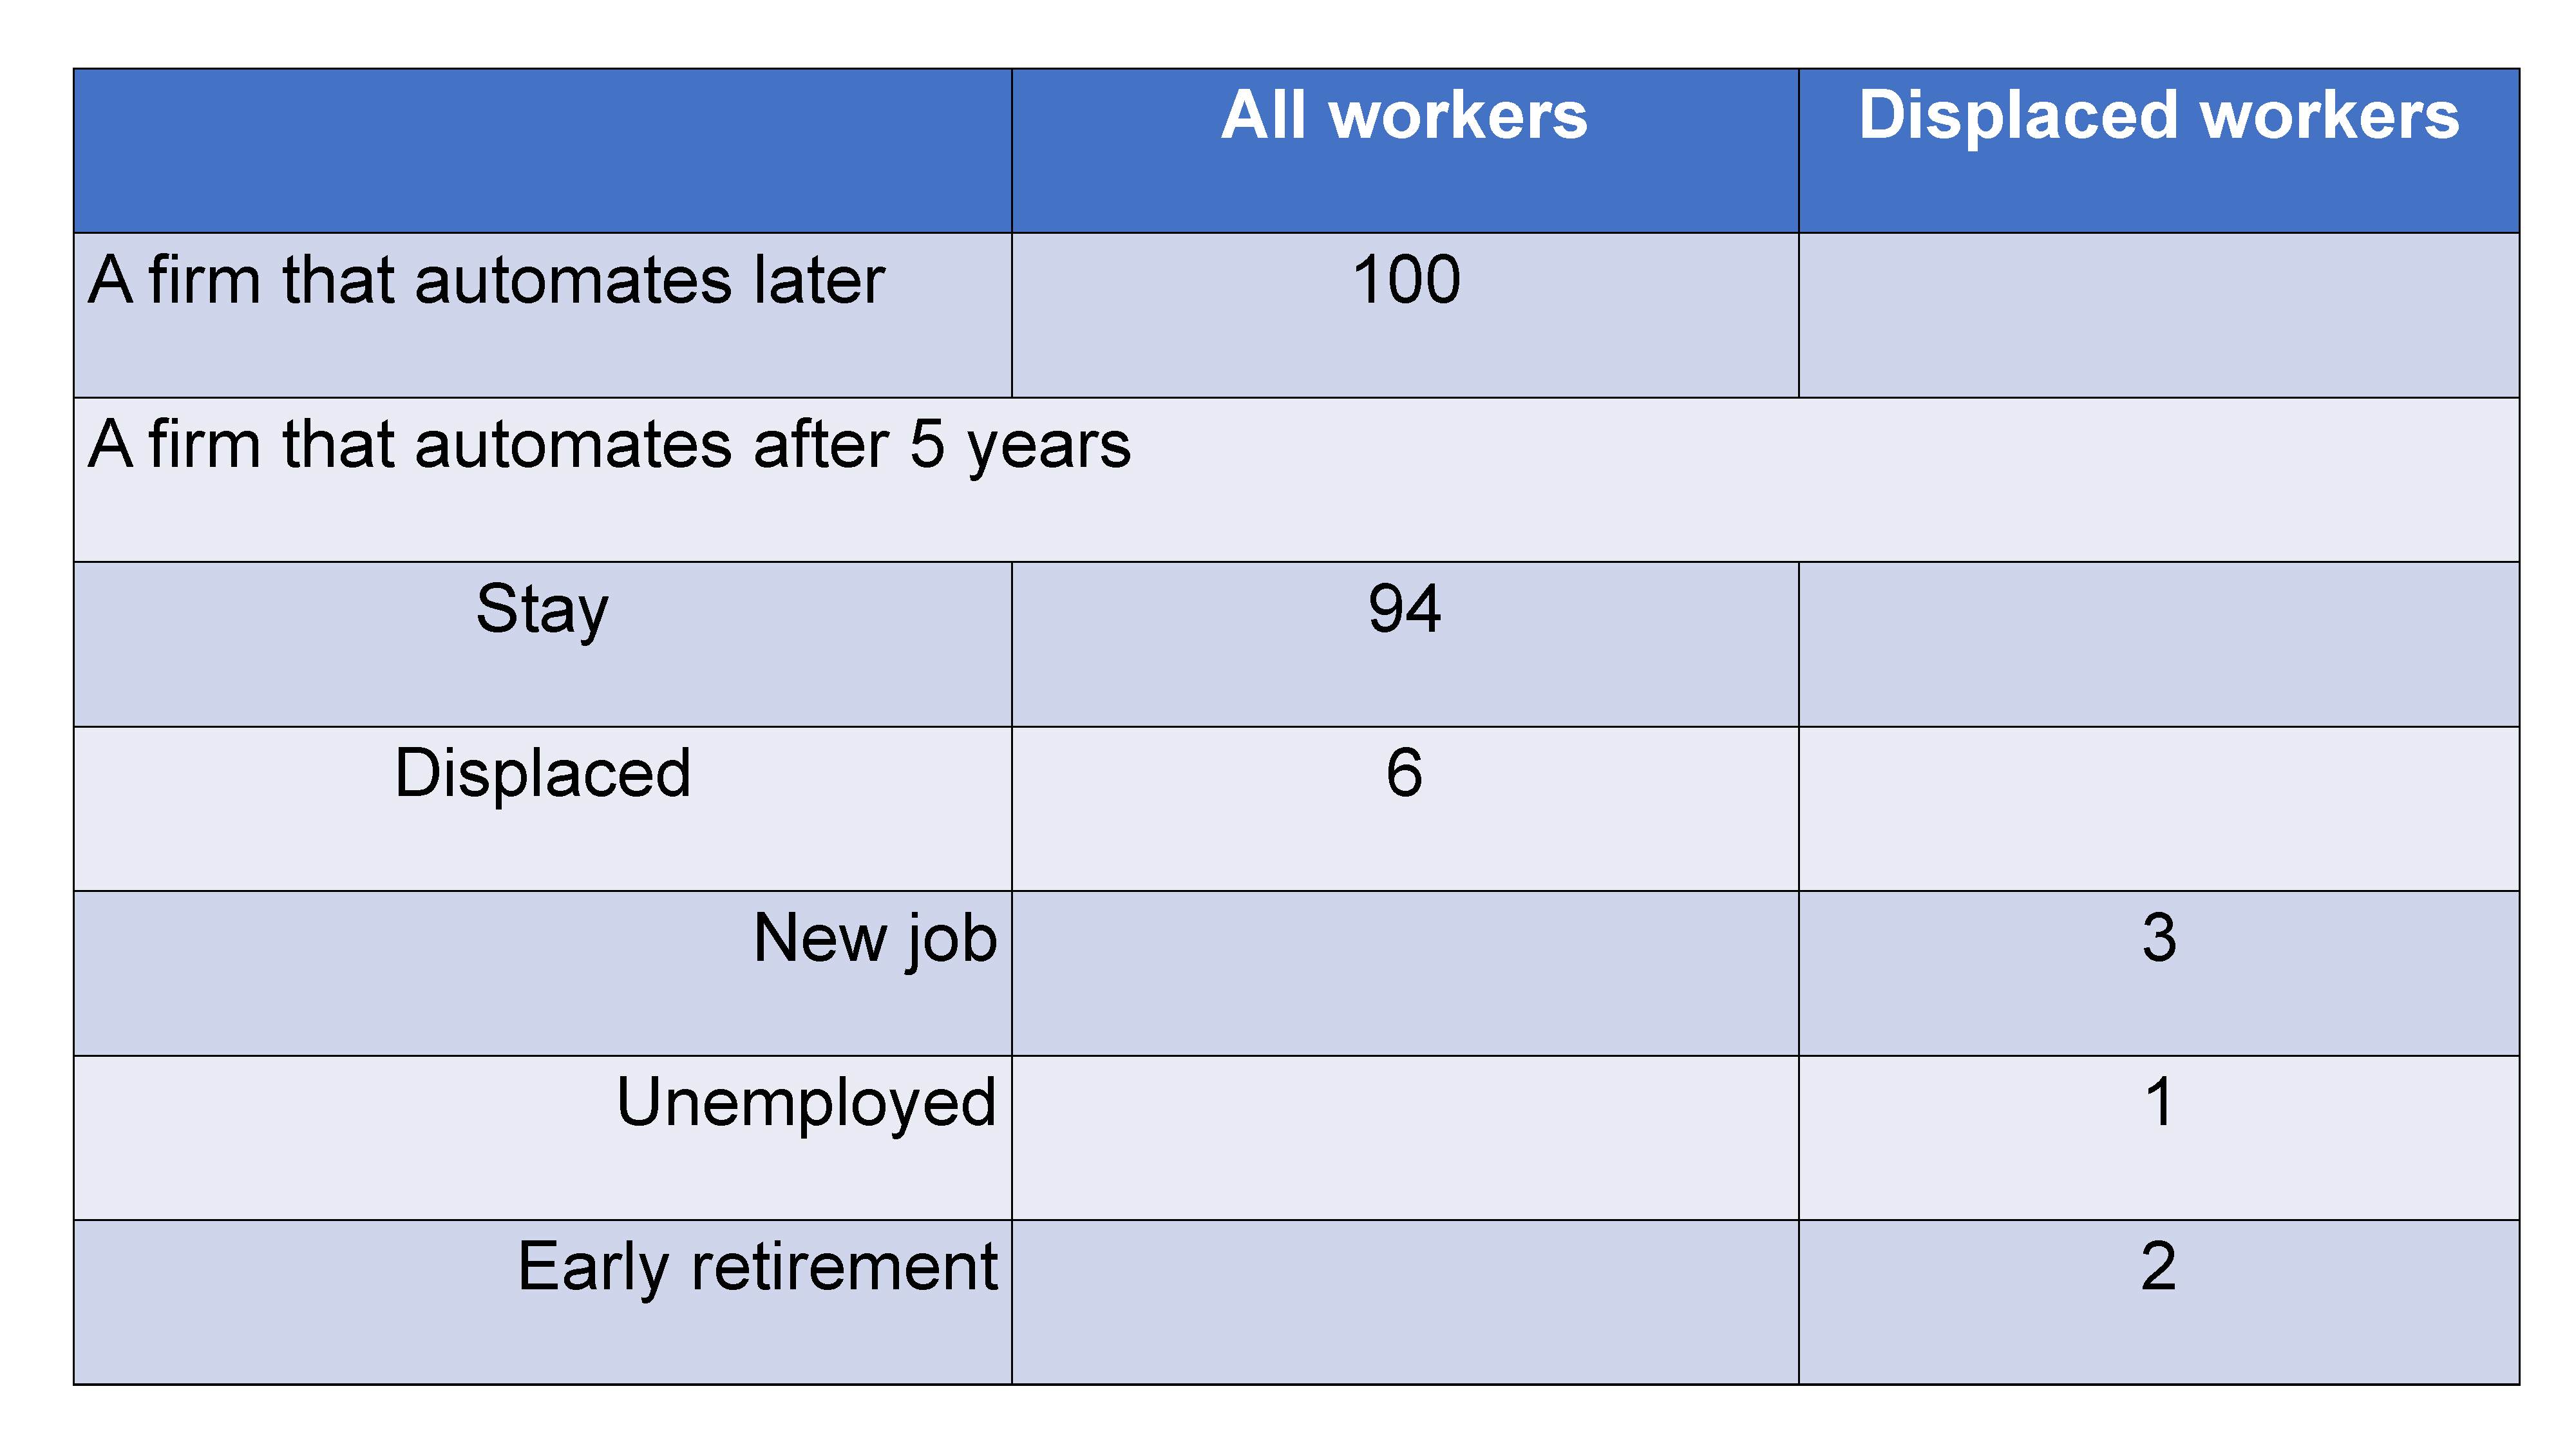
\includegraphics[width=0.9\textwidth]{figures/summary-crop.pdf}
    \end{center}
\end{frame}

\begin{frame}{Little effect on log daily wage if employed} \label{lnwage}
\noindent \begin{center}
	\includegraphics[width=0.65\paperwidth]{Paper-Revisions/graphics/w_lnwage_inc_k5_d7.PDF}
	\end{center}
\end{frame}

\begin{frame}{Effect heterogeneity} \label{heterogeneity_slide}
Annual earnings losses are: \bigskip
\begin{enumerate}
\item Pervasive across sectors \hyperlink{est_het_1}{\beamerbutton{estimates}} \bigskip
\item Larger for workers at smaller firms \hyperlink{est_het_2}{\beamerbutton{estimates}} \bigskip
\item Larger for older workers \hyperlink{est_het_2}{\beamerbutton{estimates}} \bigskip
\item Larger for less-educated workers \hyperlink{est_het_2}{\beamerbutton{estimates}} \bigskip
\item Similar for men and women \hyperlink{est_het_1}{\beamerbutton{estimates}} 
	%		\smallskip
%		\item similar by contract type \hyperlink{est_het_1}{\beamergotobutton{estimates}} Since most incumbent workers have a permanent contract anyway.
%\item Most of earnings losses are not compensated by social security benefits \hyperlink{benefits_split}{\beamergotobutton{estimates}}  
%\medskip
%\item No earnings losses for workers hired in the two years before automation event \hyperlink{recenthires}{\beamergotobutton{estimates}} 
\end{enumerate}
\end{frame}

\begin{frame}{Additional analyses} \label{additional}
\begin{itemize}
\item Other measures of employment (firm-level employment, new hires) \hyperlink{otheremp}{\beamerbutton{more}} \bigskip
\item Placebo events (investment in other material fixed assets) \hyperlink{placebo}{\beamerbutton{more}} \bigskip
\item Robustness tests (spikes, model specification, other firm-level events) \hyperlink{robustness}{\beamerbutton{more}} \bigskip
\item Clustering, FRTs, and random treatment timing \hyperlink{clustering}{\beamerbutton{more}}
\end{itemize}
\end{frame}

%%%%%%%%%%%%%%%%%%%%%%%%%%%%%%%%%%%%%%%%%%%%%%%%%%%%%%%%%%%%%%%%%%%%%%
\section{Automation versus computerization events}
%%%%%%%%%%%%%%%%%%%%%%%%%%%%%%%%%%%%%%%%%%%%%%%%%%%%%%%%%%%%%%%%%%%%%%

\begin{frame}{Computerization is less likely to decrease labor demand} \label{techspecinv}
\begin{itemize}
\item<1-> Tech progress can also be capital-augmenting \textcolor{gray}{\scriptsize{Piketty(14), Karabarbounis\&Neiman(14)}} \medskip
\item<2-> If $ F(\Psi_{K}K,L)$ with factors paid their marginal products and CRS:
\begin{equation} \nonumber
   \frac{ d \ln(W)}{d \ln(\Psi_{K})} = \frac{s^{K}}{\sigma_{KL}}  > 0 \hspace{1cm} \frac{ d \ln(s_{L})}{d \ln(\Psi_{K})} = s^{K} \left[ \frac{1}{\sigma_{KL}} -1 \right]
   \end{equation}
such that computerization must increase labor demand
\item<3-> However, a model of capital-skill complementarity: \textcolor{gray}{\scriptsize{Krusell\&al.(00)}}
\begin{equation} \nonumber
 \frac{ d W_{S}}{d \Psi_{K}} > 0 \hspace{1cm} \frac{ d W_{U}}{d \Psi_{K}} < 0 
\end{equation}
such that computerization could decrease labor demand for some workers
\end{itemize}
\end{frame}

\begin{frame}{Computerization versus automation \hyperlink{computersA}{\beamerbutton{more}}} \label{computers}
\noindent \begin{center}
	\includegraphics[width=0.65\paperwidth]{Paper-Revisions/graphics/w_relwage_inc_k5_comp.PDF}
    \end{center}
\end{frame}

%%%%%%%%%%%%%%%%%%%%%%%%%%%%%%%%%%%%%%%%%%%%%%%%%%%%%%%%%%%%%%%%%%%%%%
\section{Automation in distorted labor markets}
%%%%%%%%%%%%%%%%%%%%%%%%%%%%%%%%%%%%%%%%%%%%%%%%%%%%%%%%%%%%%%%%%%%%%%

\begin{frame}{Automation in distorted labor markets} \label{distorted}
\begin{itemize}
\item<1-> Results consistent with competitive labor markets: \bigskip   
  \begin{enumerate}
  \item \textbf{Automation $\Rightarrow$ marginal product of labor $\downarrow$} because it displaces workers more than it increases allocative efficiency \bigskip
  \item \textbf{Marginal product of labor $\downarrow$ $\Rightarrow$ $ L \downarrow$ or $W \downarrow$} because workers lack the power to benefit from increased allocative efficiency if labor markets are competitive \bigskip
  \end{enumerate}
\item<2-> If \textbf{workers have wage bargaining power}, the impact of automation on labor demand and welfare may be different \hyperlink{distorted_model}{\beamerbutton{model}} \bigskip
\item<2-> Merging collective agreements since 2000 into CBS data
\end{itemize}
\end{frame}

%%%%%%%%%%%%%%%%%%%%%%%%%%%%%%%%%%%%%%%%%%%%%%%%%%%%%%%%%%%%%%%%%%%%%%
\section{Conclusions}
%%%%%%%%%%%%%%%%%%%%%%%%%%%%%%%%%%%%%%%%%%%%%%%%%%%%%%%%%%%%%%%%%%%%%%

\begin{frame}{Conclusions}
\begin{enumerate}
\item<1-> \textbf{Automation leads to displacement} for incumbent workers \bigskip
 \item Annual earnings $\downarrow$ $\Rightarrow$ firm separation $\uparrow$ $\Rightarrow$ non-employment $\uparrow$ $\Rightarrow$ unemployment + early retirement $\uparrow$
\bigskip
%\item Affected workers more likely to \textbf{switch industries} and enter \textbf{early retirement} 
%\bigskip
\item<2-> Effects are pervasive across sectors and larger for workers in smaller firms, older workers, less-educated workers
\bigskip
\item<3-> Automation appears to be \textbf{more labor-displacing than computerization} \bigskip
\item<4-> Impact of automation may depend on \textbf{role of worker power}
\end{enumerate}
\end{frame}

%\bibliographystyle{apalike}
%\bibliography{Paper-Revisions/automation_literature}

\begin{frame}
\begin{center}
{\Large Thank you!}
\end{center}
\end{frame}

\appendix

\begin{frame}
\begin{center}
{\Large Appendices}
\end{center}
\end{frame}

\begin{frame}
\begin{center}
{\Large Appendix: New literature on automation}
\end{center}
\end{frame}

\begin{frame}{Automation and... \hyperlink{literature}{\beamerbutton{back}}} \label{otherstudies}
\begin{itemize}
    \item \textbf{the changing labor share} 
    \item[] Acemoglu\&Restrepo`20,`22; Graetz\&Michaels`18; Boustan\&al`22; Kogan\&al`21; Hubmer\&Restrepo`21; Autor\&al`20; Kehrig\&Vincent`20 
    \item \textbf{the changing occupational structure}
    \item[] Autor\&al`03; Goos\&Manning`07; Goos\&al`14; Webb`20; Kogan\&al`21; Autor\&al`22; Acemoglu\&al`22; Dillinder\&Forsythe`23
    \item \textbf{firm-level outcomes}
    \item[] Acemoglu\&al`20;Koch\&al`21;Humlum`21;Bonfiglioli\&al`22;Acemoglu\&al`23; Cheng\&al`21;Dinlersoz\&Wolf`23; Acemoglu\&al`22;Aghion\&al`23;Hirvonen\&al`22
    \item \textbf{exposed workers}
    \item[] Cortes`16, Kogan\&al`21; Feigenbaum\&Gross`20; Acemoglu\&Restrepo`20; Boustan\&al`22; Mann\&Puttmann`23, Coelli`19; Acemoglu\&Autor`11; Acemoglu\&Restrepo`22; Webb`20
\end{itemize} 
\end{frame}

\begin{frame}
\begin{center}
{\Large Appendix: Automation costs and innovation}
\end{center}
\end{frame}

\begin{frame}{Automation costs and type of innovation} \label{autom_innovation}
\begin{table}[h]
  \centering
    \begin{threeparttable}
    \begin{tabularx}{0.7\textwidth}{@{}lY@{}}
\toprule
 \multicolumn{2}{c}{\textit{Dependent variable}: Standardized automation cost share} \\
 \midrule
    Process innovations & 0.203\sym{***} \\
          & (0.048) \\
          \addlinespace
    Product innovations  & 0.098\sym{**} \\
          & (0.036) \\
          \addlinespace
    Organizational innovations  & 0.099\sym{*} \\
          & (0.041) \\
    \addlinespace
    N     & 7,160 \\
          \bottomrule
    \end{tabularx}%
    \begin{tablenotes}
           \item \emph{Notes:} Automation cost shares as a percentage of total costs, excluding automation costs. Model controls for one-digit industry fixed effects and the log number of workers at the firm, and is weighted by survey weights.
           \end{tablenotes}
          \end{threeparttable}
\end{table}%
\end{frame}

\begin{frame}{Automation costs and technology usage \hyperlink{data}{\beamerbutton{back}}}
\begin{table}[h]
\footnotesize
  \scalebox{0.6}{
    \begin{threeparttable}
    \begin{tabularx}{1.4\textwidth}{@{}lYllY@{}}
\toprule
 \multicolumn{5}{c}{\textit{Dependent variable}: Standardized automation cost share} \\
 \midrule
    Use of electronic data suited to automated processing & 0.236\sym{***} &       & Received orders for goods or services through EDI & 0.106\sym{**} \\
          & (0.053) &       &       & (0.0339) \\
    N     & 4,313 &       & Ordered through Electronic Data Interchange (EDI) & -0.099\sym{**} \\
          &       &       &       & (0.032) \\
    CRM, inventory and distribution analysis & 0.200\sym{***} &       & N     & 14,172 \\
          & (0.041) &       &       &  \\
    Customer Relationship Mngmnt (CRM), customer analysis & 0.055 &       & Sales software & 0.088\sym{**} \\
          & (0.048) &       &       & (0.030) \\
    N     & 11,927 &       & Purchasing software & 0.006 \\
          &       &       &       & (0.03) \\
    Enterprise Resource Planning (ERP) software & 0.164\sym{***} &       & N     & 7,831 \\
          & (0.027) &       &       &  \\
    N     & 12,535 &       & Radio Frequency Identification (RFID) & 0.056 \\
          &       &       &       & (0.083) \\
    Automated records used for value chain integration & 0.200\sym{**} &       & N     & 4,149 \\
          & (0.066) &       &       &  \\
    Value chain integration & -0.008 &       & Local Area Network (LAN) & 0.015 \\
          & (0.047) &       &       & (0.026) \\
    N     & 7,879 &       & N     & 7,653 \\
          &       &       &       &  \\
    Big data analysis & 0.127\sym{*} &       & Internet for financial transactions & 0.016 \\
          & (0.054) &       &       & (0.025) \\
    N     & 4,680 &       & N     & 7,526 \\
          &       &       &       &  \\
    Cloud-services: Software for customer information mngmnt & 0.168\sym{*} &       & Internet for training and education (incl. e-learning) & 0.035 \\
          & (0.084) &       &       & (0.031) \\
    Cloud-services: Software for accounting and financial mngmnt & 0.136\sym{*} &       & N     & 8,385 \\
          & (0.062) &       &       &  \\
    N     & 6,711 &       &       &  \\
          \bottomrule
    \end{tabularx}%
          \end{threeparttable}
          }
\end{table}%
\end{frame}

\begin{frame}
\begin{center}
{\Large Appendix: Automation costs and automation imports} \label{comp_imports}
\end{center}
\end{frame}

%We also observe average imports of robots and other automation technology for a subset of firms in our data\footnote{Consistent import data only start in 2010, so we construct firm-level averages and remove firms which cease operations before 2009 when comparing our automation cost data to automation imports. Details on import data can be found in Appendix \ref{}.}. Automation imports are defined as imports of intermediates classified by \citet{Acemoglu2019b} as robots, numerically controlled machines, automatically controlled machines, automatic transfer machines, and automatic welding machines. Net imports are defined as imports minus re-exports. Table \ref{sumstat_imports_sector} compares these two measures as a share of total operating cost for the overlapping subsample at the sector level, revealing that automation expenditures are substantially higher than automation imports -- since few firms are importers--, and observed across a wider range of sectors. However, automation imports and automation expenditures are correlated at the firm-level, as shown in Table \ref{sumstat_imports_firm} where firm-level automation expenditures are regressed onto (net) automation imports while controlling for firms' total operating cost. This comparison validates our measure as being correlated to the import measures often used in the literature, while also showing its broader coverage across sectors and firms.

%% Story here
% For all firms from 2010 onwards, we also observe average imports of robots and other automation technologies. 
%Automation imports = imports of intermediates, in classification of Acemoglu-Restrepo 2019 (so distinguish between robots, numerically controlled machines, automatically controlled machines, automatic transfer machines and automatic welding machines.)

% This table compares automation costs and imports as a share of total costs per sector. First we see that: automation expenditures are substantially higher than imports, since few firms are importers [How many?]. ALso substantial re-exports. Might be a Dutch thing, with a lot of trading companies, but its probable that those re-exporting them, are not using the machines.
% Automation costs are observed across a wider range of sectors than imports.
% However, they are correlated at the firm-level, which is shown in the second table. Here we regress firm-level automation expenditures onto automation ports while controlling for total operating costs. 
% So, our measure is correlated to the import measures often used in the literature, but alsos shows broader coverage across sectors and firms.

\begin{frame}{Comparing automation costs to automation imports by sector} \label{sumstat_imports_sector}
\begin{table}[h]
\footnotesize
  \centering
  %\caption{Comparing automation costs to automation imports by sector} \label{sumstat_imports_sector}
      \begin{threeparttable}
    \begin{tabularx}{0.8\textwidth}{@{}lYYY@{}}
    \toprule
    \addlinespace  
          & \multicolumn{3}{c}{\textbf{Mean share in total costs}}   \\
   	\textbf{Sector}  & Automation costs & Imports & Net imports \\
   \midrule
    Manufacturing & 0.346 & 0.081 & 0.043 \\
    Construction & 0.193 & 0.001 & 0.001 \\
    Wholesale \& retail trade & 0.300 & 0.058 & 0.051 \\
    Transportation \& storage & 0.353 & 0.134 & 0.095 \\
    Accommodation \& food serving & 0.268 & 0.000 & 0.000 \\
    Information \& communication & 0.804 & 0.004 & 0.004 \\
    Prof'l, scientific \& technical activities & 1.006 & 0.007 & 0.005 \\
    Administrative \& support activities & 0.437 & 0.003 & 0.003 \\
    \bottomrule
    \end{tabularx}%
    \begin{tablenotes}
           \item \emph{Notes:} Total N firms is 30,267. Net automation imports are defined as imports minus re-exports. \\ Total costs include automation costs. 
           \end{tablenotes}
          \end{threeparttable}
\end{table}%
\end{frame}

\frame{\frametitle{Comparing automation costs to automation imports at the firm level}
\begin{table}[h]
  \centering
 % \caption{Comparing automation costs to automation imports \\ between and within firms} \label{sumstat_imports_firmyear}

    \begin{threeparttable}
    \footnotesize
    \begin{tabularx}{0.8\textwidth}{@{}lYYYY@{}}
    \toprule
    \addlinespace  
    \multicolumn{5}{c}{\textit{Dependent variable:} Automation costs (IHS)}   \\
    \midrule
    & (1) & (2) & (3) & (4) \\
    \cmidrule{2-5} 
    Automation imports (IHS) & 0.0178\sym{**} & 0.0177\sym{**} & -0.001 & -0.002 \\
          & (0.007) & (0.007) & (0.004) & (0.004) \\
    \addlinespace
    \addlinespace
     & (5) & (6) & (7) & (8) \\
    \cmidrule{2-5} 
    \addlinespace
    Net automation imports (IHS) & 0.0158\sym{*} & 0.0157\sym{*} & -0.003 & -0.003 \\
          & (0.006) & (0.006) & (0.004) & (0.004) \\
    \addlinespace
    \hline \hline
    \addlinespace
    Year fixed effects & No & Yes & No & Yes \\
    Firm fixed effects & No & No & Yes & Yes \\
    Log total costs & Yes & Yes & Yes & Yes \\
    \bottomrule
    \end{tabularx}%
    \begin{tablenotes}
           \item \emph{Notes:} $N$=110,698 (firm-year). Automation costs, imports, and net imports are transformed using the inverse hyperbolic sine (IHS). Net automation imports are defined as imports minus re-exports. All models control for log total costs at the firm-year level. Standard errors are clustered at the firm-level.
           \end{tablenotes}
          \end{threeparttable}
    
\end{table}%
}

\frame{\frametitle{Importers are much larger than firms with automation events}
\begin{table}
\begin{threeparttable}
    \begin{tabularx}{0.8\textwidth}{@{}lYYcYY@{}}
    \multicolumn{6}{c}{\textit{Dependent variable:} Log firm-level number of employees} \\
\toprule
          & \multicolumn{2}{c}{Automation cost spike} &       & \multicolumn{2}{c}{Automation imports} \\
          & (1)   & (2)   &       & (3)   & (4) \\
          \cmidrule(l{0pt}r{0pt}){2-3} \cmidrule(l{0pt}r{0pt}){5-6}
    Automating & 0.078\sym{***} & 0.085\sym{***} &       & 0.857\sym{***} & 0.838\sym{***} \\
          & (0.013) & (0.013) &       & (0.022) & (0.022) \\
\noalign{\vskip 2mm} 
    Sector fixed effects & No    & Yes   &       & No    & Yes \\
\bottomrule 
\end{tabularx}%
\begin{tablenotes}
 \item \emph{Notes:} N = 30,267 firm-level observations. Automation imports measured as non-zero mean automation imports at the firm level. Sector fixed effects are two-digit sector dummies. *p$<$0.10, **p$<$0.05, ***p$<$0.01.
\end{tablenotes}
\end{threeparttable}
\end{table}%
}

\frame{\frametitle{Between firms: automation events and automation importer correlation}
\begin{table}
  \centering
\begin{threeparttable}
    \begin{tabularx}{0.8\textwidth}{@{}lYYYY@{}}
\toprule
          \multicolumn{5}{c}{\textit{Dependent variable:} Dummy for firm having an automation cost spike} \\
          & (1)   & (2)   & (3)   & (4) \\
   	 \cmidrule{2-5}
    Importer & 0.022\sym{*} & 0.028\sym{**} &       &  \\
          & (0.010) & (0.011) &       &  \\
    Net importer &       &       & 0.022\sym{*} & 0.028\sym{**} \\
          &       &       & (0.010) & (0.011) \\
    \addlinespace      
    Controls  & No    & Yes   & No    & Yes \\
\bottomrule 
\end{tabularx}%
\begin{tablenotes}
 \item \emph{Notes:} N = 30,267 firm observations, where 31\% of firms have automation cost spikes, and 8.2\% (7.9\%) have non-zero (net) imports. Controls are log total costs and sector fixed effects. Standard errors are clustered at the firm-level. *p$<$0.10, **p$<$0.05, ***p$<$0.01.
\end{tablenotes}
\end{threeparttable}
\end{table}%
}

\frame{\frametitle{Within firms: automation events and automation importers \hyperlink{data}{\beamerbutton{back}}}
\begin{table}
  \centering
\begin{threeparttable}
    \begin{tabularx}{0.9\textwidth}{@{}lYYYY@{}}
\toprule
          \multicolumn{5}{c}{\textit{Dependent variable:} Dummy for firm having an automation cost spike} \\
    \midrule      
          & (1)   & (2)   & (3)   & (4) \\
   	 \cmidrule{2-5}
    Importer & 0.005 & 0.002 & 0.003 & 0.000 \\
          & (0.005) & (0.005) & (0.005) & (0.005) \\
    \addlinespace
          & (5)   & (6)   & (7)   & (8) \\
       	 \cmidrule{2-5}
    Net importer & 0.003 & 0.000 & 0.001 & -0.001 \\
          & (0.005) & (0.005) & (0.005) & (0.005) \\
\addlinespace
\hline \hline
\addlinespace
    Firm fixed effects & Yes   & Yes   & Yes   & Yes  \\
    Year fixed effects & No    & Yes   & No    & Yes \\
    Log total costs & No    & No    & Yes   & Yes \\
\bottomrule 
\end{tabularx}%
\begin{tablenotes}
 \item \emph{Notes:} N = 110,698 firm-year observations. Standard errors are clustered at the firm-level. *p$<$0.10, **p$<$0.05, ***p$<$0.01.
\end{tablenotes}
\end{threeparttable}

\end{table}%
}

\begin{frame}
\begin{center}
{\Large Appendix: Data cleaning}
\end{center}
\end{frame}

\begin{frame}{Data cleaning \hyperlink{data}{\beamerbutton{back}}} \label{data_cleaning}
We remove the following observations:
\medskip
\begin{itemize}
\item Workers enrolled in full-time studies earning either less than EUR 5K  annually or EUR 10 daily on average across the year
\medskip
\item Workers with earnings above EUR 500K annually or EUR 2K daily on average across the year
\medskip
\item Later, we further exclude workers at firms that have:
\begin{itemize}
\item Not a single spike in automation cost shares \smallskip
\item No event window (7 yrs of consecutive data) \smallskip
\item Other events in the event window (mergers, takeovers, splits, restructuring) \smallskip
\item Large ($>$90\%) annual employment changes in the event window or also outside the event window
\smallskip
\end{itemize}
\end{itemize}
\end{frame}

\begin{frame}
\begin{center}
{\Large Appendix: Descriptive statistics on automation costs}
\end{center}
\end{frame}

\begin{frame}{Distribution of automation costs \hyperlink{des_autom_time}{\beamerbutton{back}}} \label{des_autom}
\footnotesize
\noindent \begin{table}[t!]
  \centering
    \begin{threeparttable}
    \begin{tabular}{lcccccc}
    \toprule
    \addlinespace
          & \multicolumn{3}{c}{\textbf{All observations}} & \multicolumn{3}{c}{\textbf{Automation costs $>0$}} \\
          & Cost  & Cost  & Cost  & Cost  & Cost  & Cost \\
          & level & per worker & share (\%) & level & per worker & share (\%) \\
    \midrule      
    p5    & 0     & 0     & 0     & 2,211 & 59    & 0.04 \\
    p10   & 0     & 0     & 0     & 3,987 & 101   & 0.06 \\
    p25   & 0     & 0     & 0     & 10,487 & 256   & 0.14 \\
    p50   & 11,736 & 283   & 0.16  & 30,000 & 641   & 0.32 \\
    p75   & 52,824 & 986   & 0.47  & 93,711 & 1,447 & 0.68 \\
    p90   & 192,393 & 2,256 & 1.06  & 305,111 & 2,949 & 1.37 \\
    p95   & 453,172 & 3,625 & 1.69  & 713,121 & 4,590 & 2.13 \\
    \textit{mean} & \textit{211,326} & \textit{1,045} & \textit{0.44} & \textit{307,840} & \textit{1,522} & \textit{0.64} \\
          &       &       &       &       &  \\
    \multicolumn{1}{l}{N firms $\times$ years} & \multicolumn{3}{c}{238,623} & \multicolumn{3}{c}{163,810} \\
    N with 0 costs & \multicolumn{3}{c}{31\%} & \multicolumn{3}{c}{0\%} \\
    \bottomrule
    \end{tabular}%
  \end{threeparttable}
\end{table}
\end{frame}

\begin{frame}
\begin{center}
{\Large Appendix: Automation cost spike frequences}
\end{center}
\end{frame}

\begin{frame}{Automation cost spike frequencies \hyperlink{spike}{\beamerbutton{back}}} \label{spikefrequency}
\footnotesize
\begin{table}[t!]
  \centering
    \begin{threeparttable}
    \begin{tabular}{lcc}
    \toprule
    \textbf{Spike frequency} & \textbf{N firms} & \textbf{\% of N firms} \\
    \midrule
    0     & 25,145 & 70.7 \\
    1     & 8,351 & 23.5 \\
    2     & 1,772 & 5.0 \\
    3     & 266   & 0.7 \\
    4     & 29    & 0.1 \\
    5     & 4     & 0.0 \\
    Total & 35,567 & 100 \\
    \bottomrule
    \end{tabular}%
    \begin{tablenotes}
           \item \emph{Notes:} Spike frequency is defined as the total number of spikes occurring over 2000-2016. The total number of firms is 35,567 and the total number of firms with at least one automation cost share spike is 10,422.
           \end{tablenotes}
          \end{threeparttable}
\end{table}%
\end{frame}

\begin{frame}
\begin{center}
{\Large Appendix: A model of monopolistic competition with endogenous automation}
\end{center}
\end{frame}

\begin{frame}{Consumption and product demand} \label{modelA}
\begin{itemize}
    \item Utility is given by:
    \begin{equation} \nonumber
    U(Y_{1},...,Y_{J})= \left[ \sum_{j=1}^{J} [ \epsilon_{j}Y_{j}]^{\frac{\sigma-1}{\sigma}} \right]^\frac{\sigma}{\sigma-1} \text{ such that } \sum_{j=1}^{J} P_{j}Y_{j} = P Y \label{eq_CES_utility}
    \end{equation}
    where $ \sigma >1$
    \item The ideal price index given by:
    \begin{equation} \nonumber
    P(P_{1},...,P_{J}) \equiv \left[ \sum_{j=1}^{J} [P_{j}/ \epsilon_{j}]^{1-\sigma} \right]^\frac{1}{1-\sigma} = 1 \label{eq_CES_ideal_price_index}
    \end{equation}
    \item Demand for firm $j$ is given by:
    \begin{equation} \nonumber
    Y_{j} = Y \epsilon_{j}^{\sigma - 1} P_{j}^{-\sigma} \label{eq_CES_demand}
    \end{equation}
\end{itemize}    
\end{frame}

\frame{\frametitle{Firm-level allocation of capital and labor across tasks in production} 
\noindent \begin{center}
	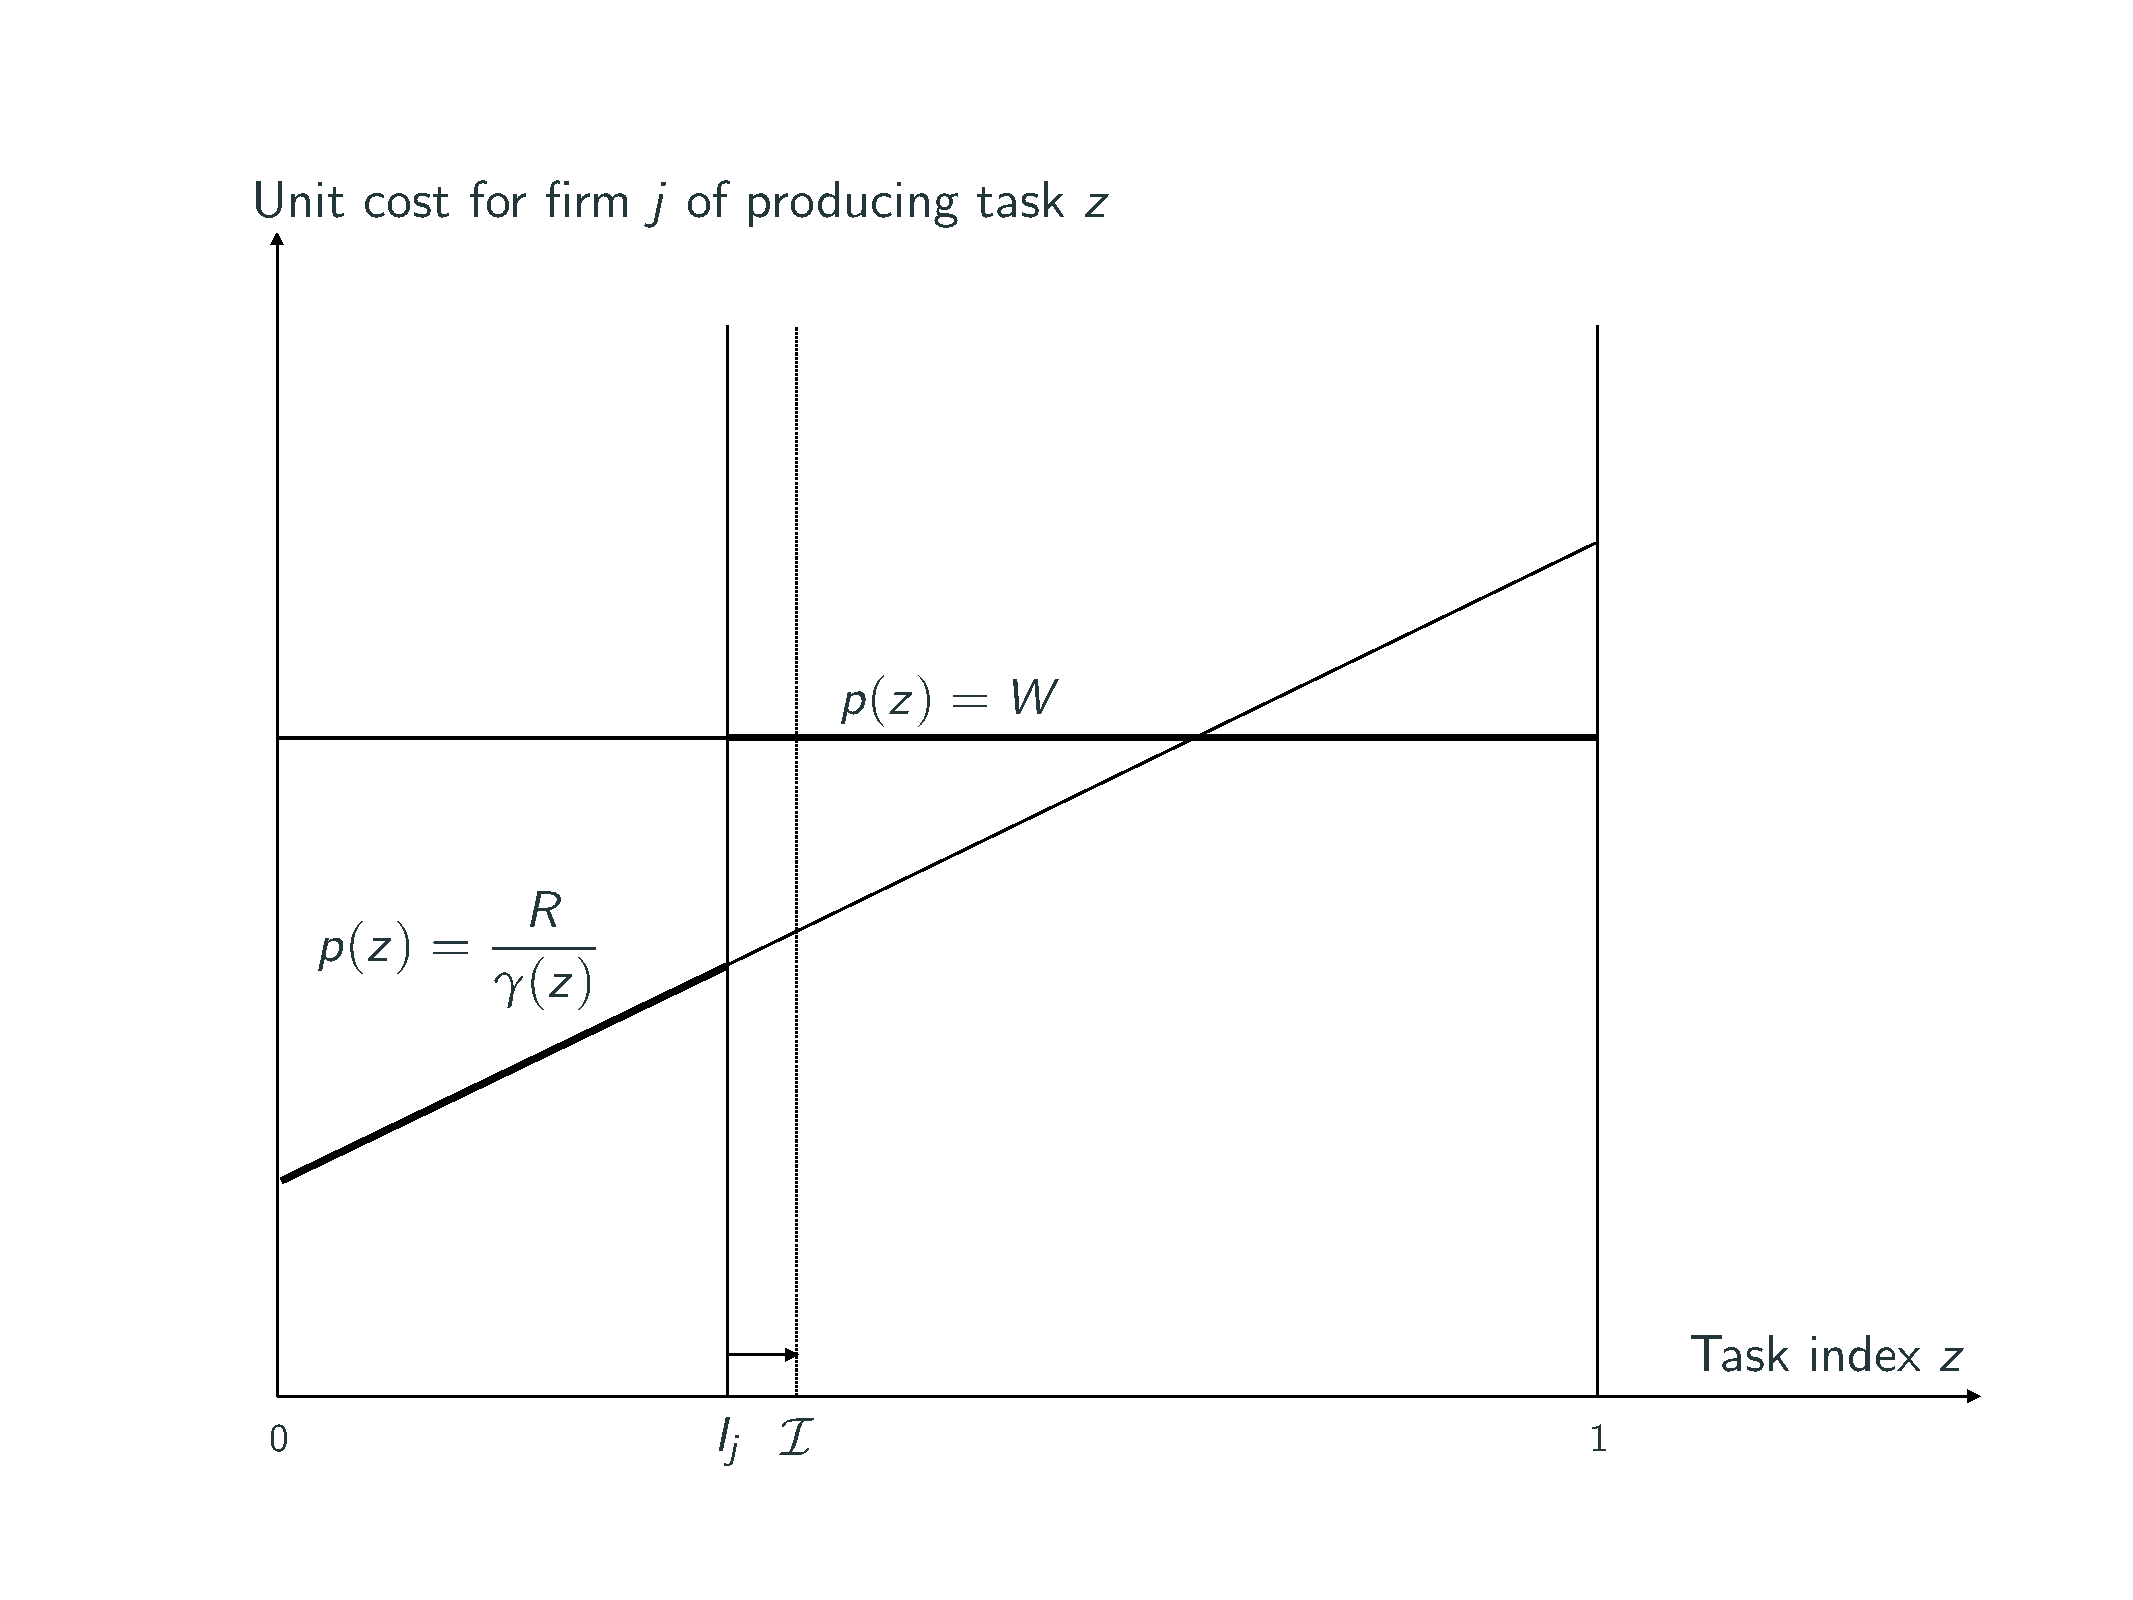
\includegraphics[width=0.6\paperwidth]{figures/figure1.pdf}
    \end{center}
}

\frame{ \frametitle{Factor bills, prices, output, and profits \hyperlink{model}{\beamerbutton{back}}}
\begin{itemize}
    \item Conditional factor demands are given by:
    \begin{equation} \nonumber
    RK_{j} = I_{j} \frac{\sigma - 1}{\sigma} P_{j}Y_{j} \text{\hspace{0.2cm} and \hspace{0.2cm}} WL_{j} = [1-I_{j}] \frac{\sigma - 1}{\sigma} P_{j}Y_{j}
    \end{equation}
    \item The (relative) output price is given by:
    \begin{equation} \nonumber
    P_{j} = \frac{\sigma}{\sigma-1} \frac{W^{1-I_{j}} R^{I_{j}}}{\Psi_{H}(I_{j})}
    \end{equation}
    \item Output is given by:
    \begin{equation} \nonumber
    Y_{j} = Y \epsilon_{j}^{\sigma-1} P_{j}^{- \sigma} = Y \epsilon_{j}^{\sigma-1} \left[ \frac{\sigma}{\sigma-1} \frac{W^{1-I_{j}} R^{I_{j}}}{\Psi_{H}(I_{j})} \right]^{- \sigma} 
    \end{equation}
    \item Profits are given by:
    \begin{equation} \nonumber
    \Pi_{j} = \frac{P_{j}Y_{j}}{\sigma}
\end{equation}
\end{itemize}
}

\begin{frame}
\begin{center}
{\Large Appendix: Forbidden comparisons}
\end{center}
\end{frame}

\begin{frame}{Time-varying homogeneous effects} \label{forbidden} 
\noindent \begin{center}
	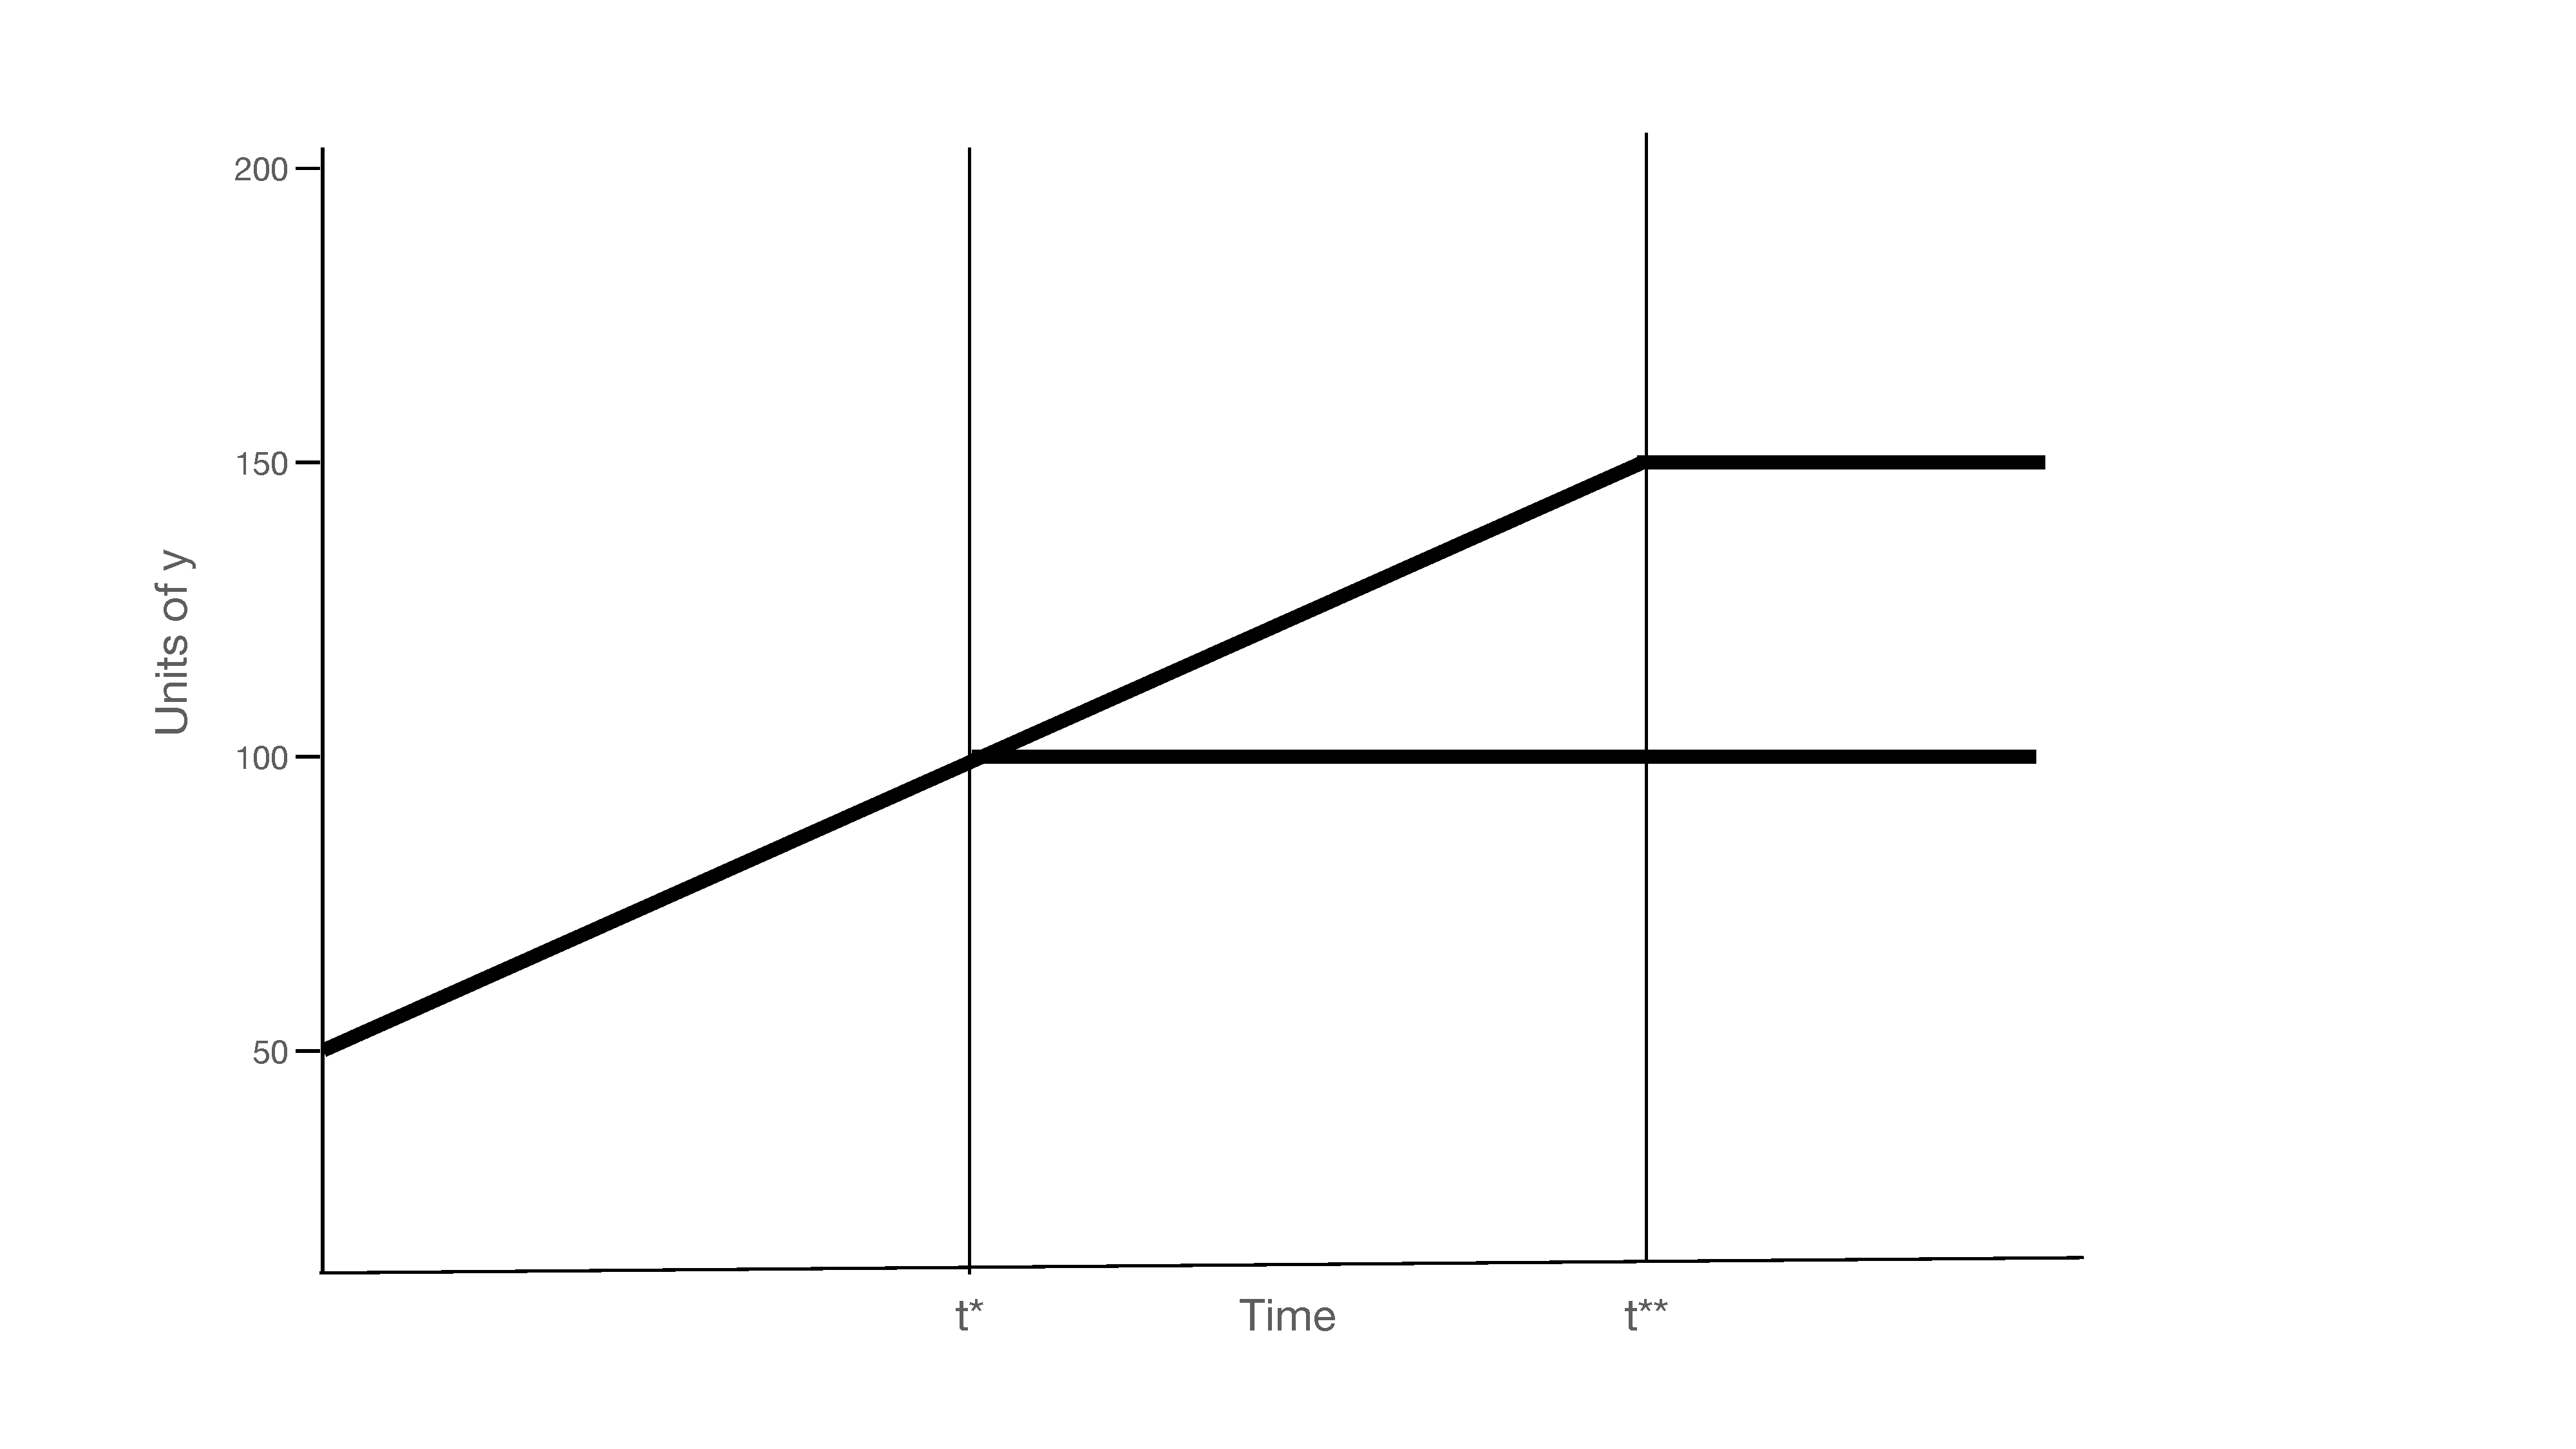
\includegraphics[width=0.7 \paperwidth]{figures/forbidden1.pdf}
    \end{center}
\end{frame}

\frame{\frametitle{Good comparisons}
\noindent \begin{center}
	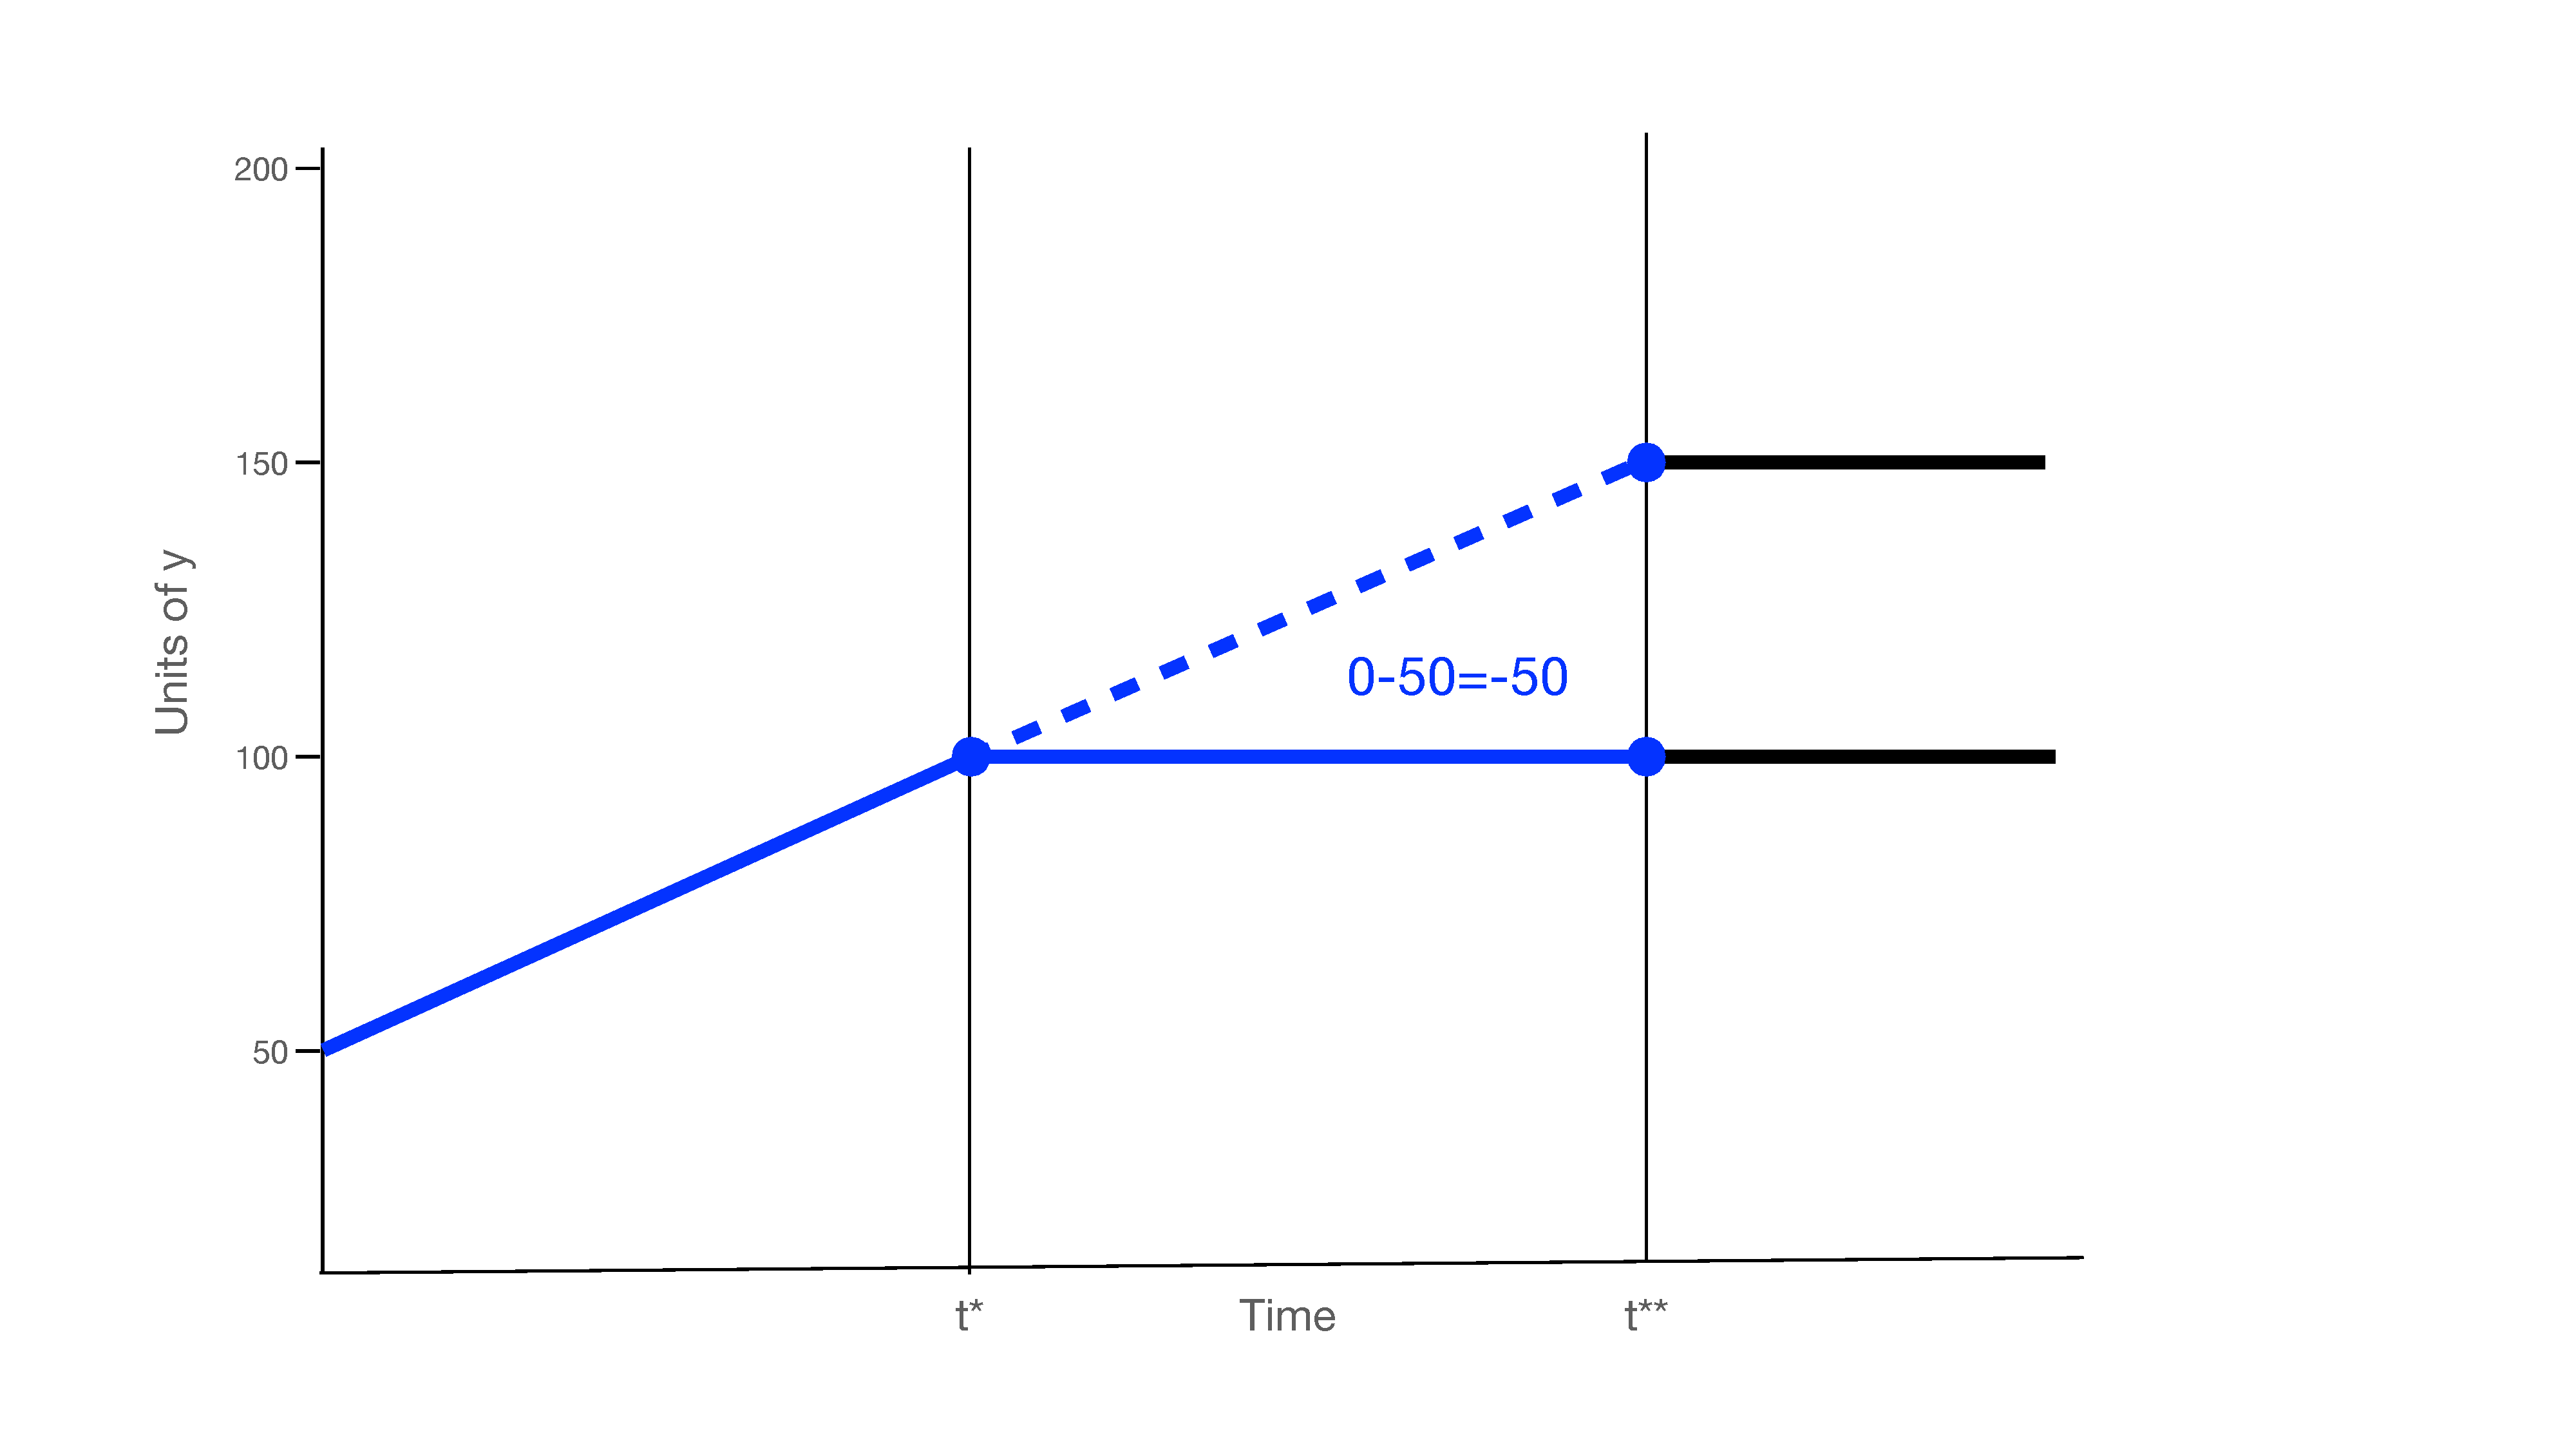
\includegraphics[width=0.7 \paperwidth]{figures/forbidden2.pdf}
    \end{center}
}

\frame{\frametitle{Forbidden comparisons \hyperlink{twfe}{\beamerbutton{back}}}
\noindent \begin{center}
	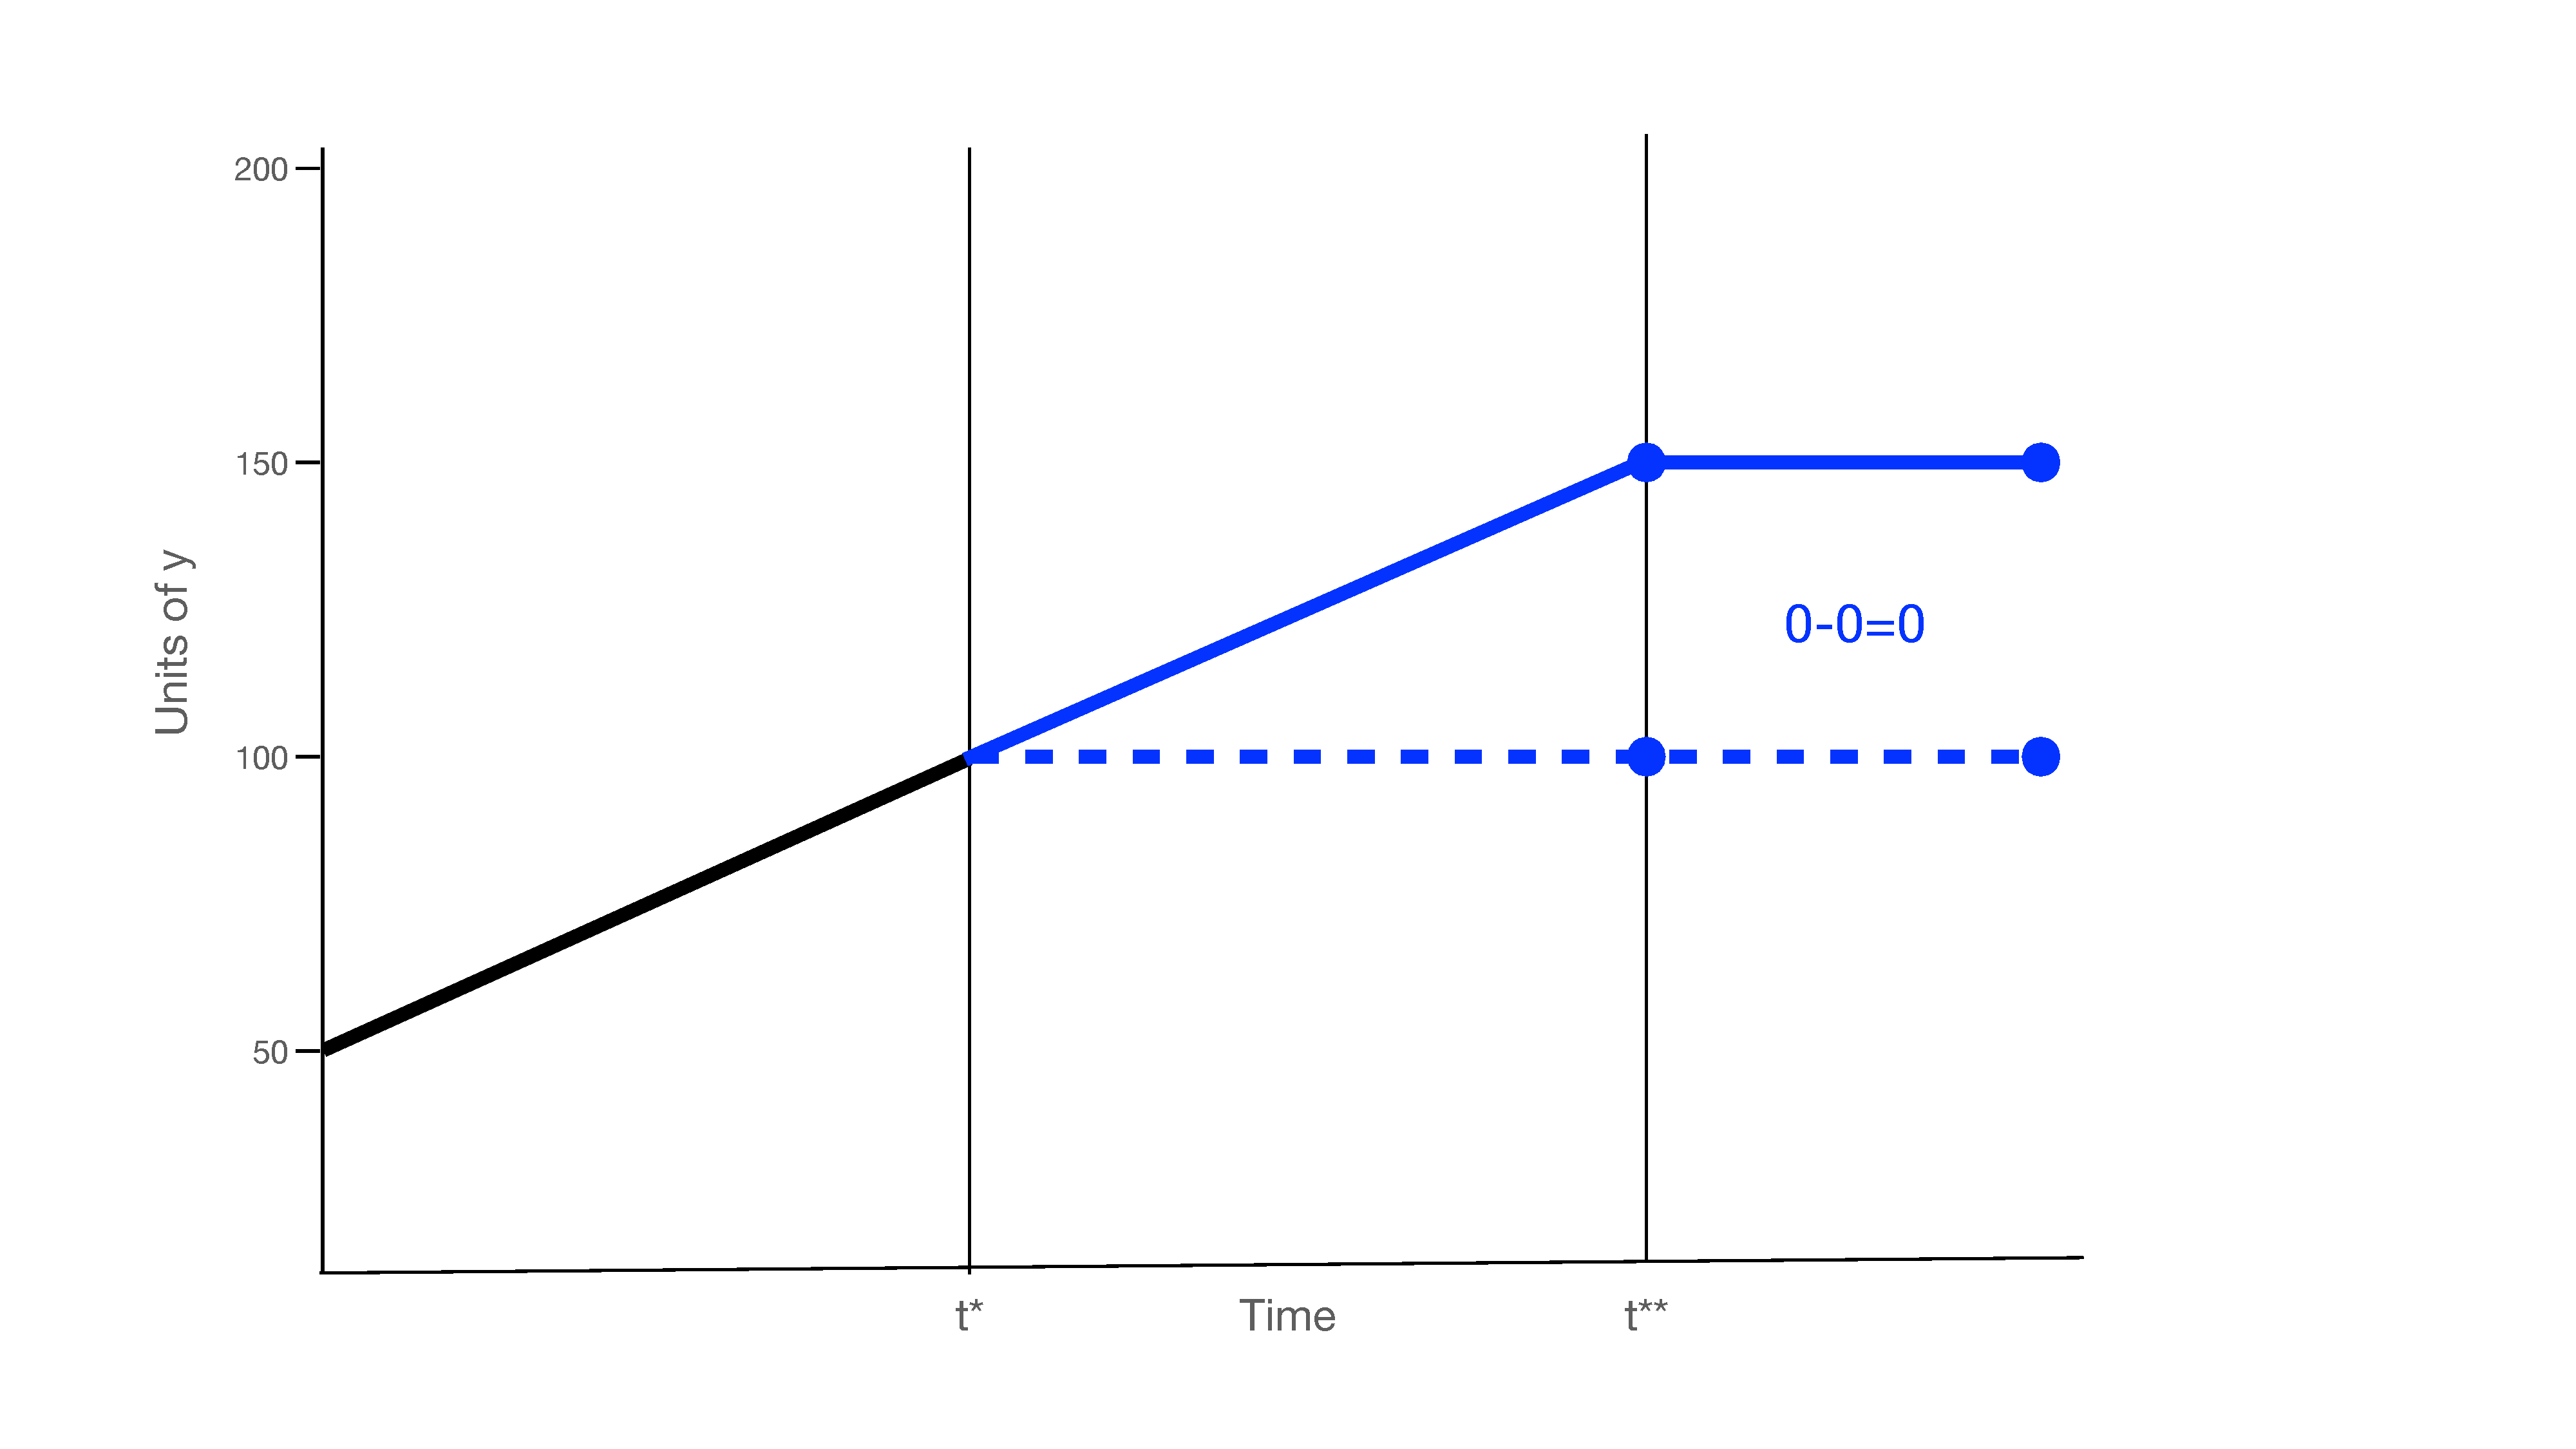
\includegraphics[width=0.7 \paperwidth]{figures/forbidden3.pdf}
    \end{center}
}

\begin{frame}
\begin{center}
{\Large Appendix: Other estimators for staggered DiD designs}
\end{center}
\end{frame}

\begin{frame}{Other estimators for staggered DiD designs} \label{otherest} 
\begin{enumerate}
    \item \textbf{Callaway\&Sant'Anna} (\texttt{csdid}): doubly robust estimator, flexible aggregation, covariates, bootstrapping, simultaneous CI \medskip
    \item \textbf{Sun\&Abraham} (\texttt{eventstudyinteract}): 3-step estimator, Interaction-Weighted regression, event-studies  \medskip
    \item \textbf{Chaisemartin\&D'Haultfoeuille} (\texttt{did\_multiplegt\_dyn}):  Wald-TC estimator of treatment effects on switchers, instantaneous treatment effects, non-staggered designs, multi-valued treatments \medskip
    \item \textbf{Roth\&Sant'Anna} (\texttt{staggered}): general DiD/DiM plugin estimator, efficient estimator if treatment timing is random \medskip
    \item \textbf{Borusyak\&al.} (\texttt{did\_imputation}): 3-step imputation estimator (\texttt{event\_plot} for plotting event-study graphs)  \medskip
\end{enumerate}
For an overview, go to \href{https://asjadnaqvi.github.io/DiD/}{https://asjadnaqvi.github.io/DiD/}
\end{frame}

\frame{\frametitle{Other estimators for staggered DiD designs \hyperlink{twfe}{\beamerbutton{back}}}
\noindent \begin{center}
	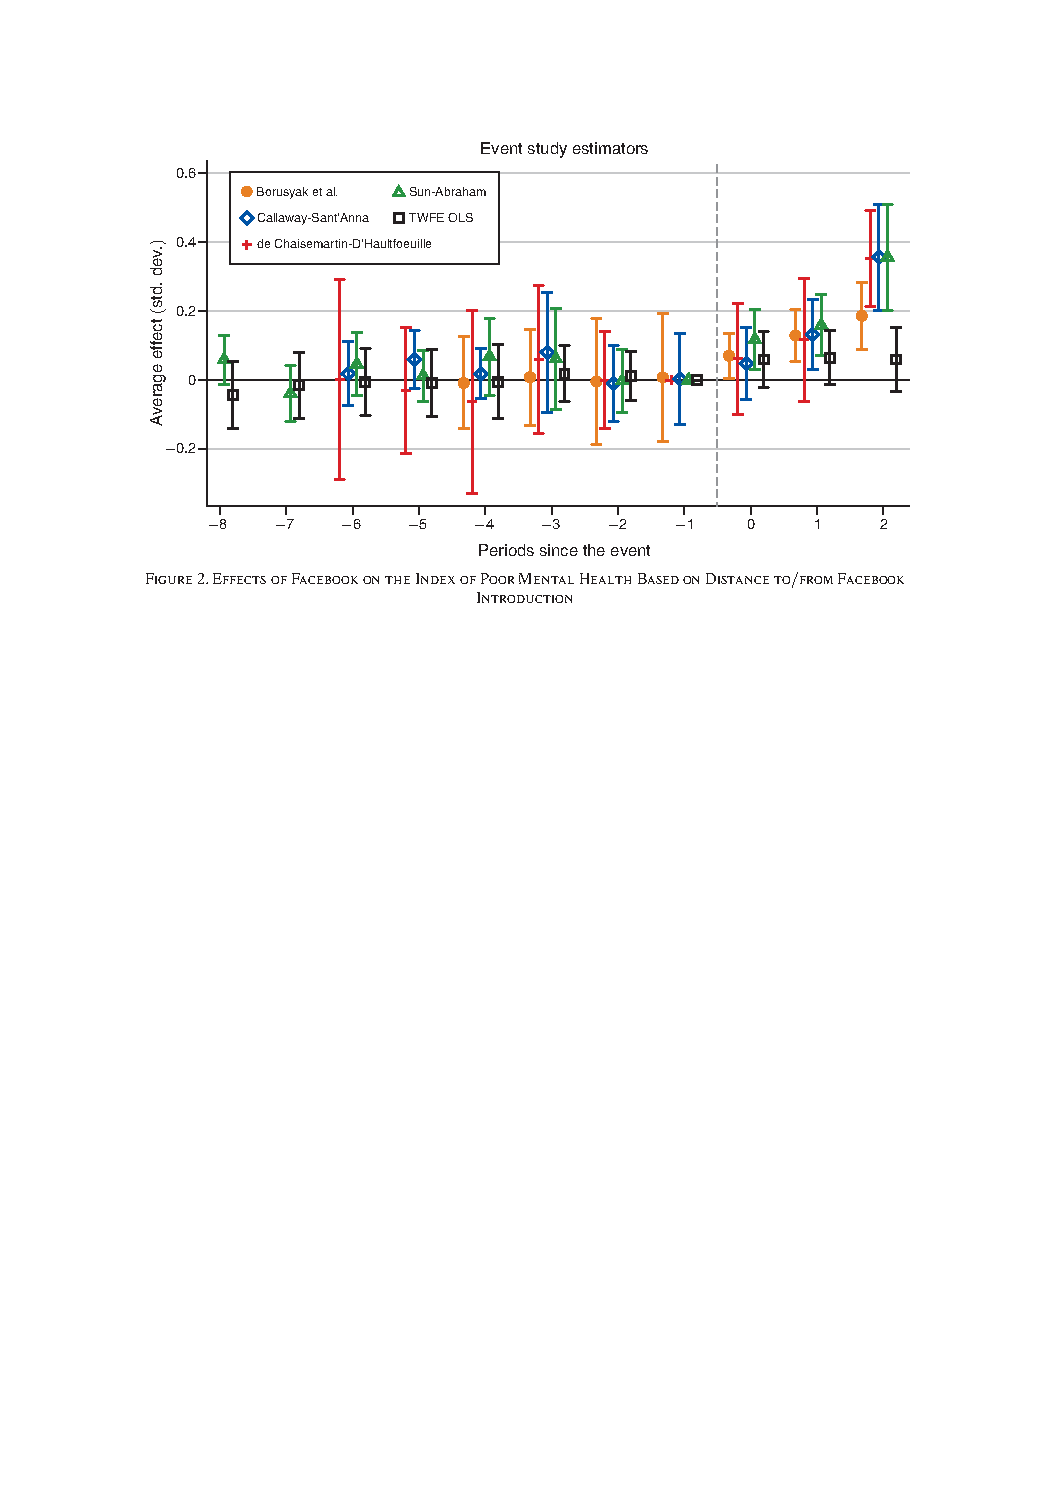
\includegraphics[width=0.7 \paperwidth]{figures/estimators.pdf}
    \end{center}
\footnotesize{Braghieri\&al.'22, ``Social Media and Mental Health", \textit{American Economic Review} 2022, 112(11)}
}

\begin{frame}
\begin{center}
{\Large Appendix: Matching details}
\end{center}
\end{frame}

\begin{frame}{CEM statistics \hyperlink{treatment}{\beamerbutton{back}}} \label{CEM_stats}
\begin{itemize}
\item Coarsened Exact Matching (CEM): \medskip
\begin{enumerate}
\item In each of the three pre-treatment years, separate strata for each 5 percentiles of annual wage + separate bins for the 99th and 99.5th percentiles \medskip
\item One year prior to treatment, matched workers must be observed in the same calendar year and work in the same sector
\end{enumerate} \medskip
\item 30,247 strata \medskip
\item 98\% of treated incumbents are matched; and 93\% of control group incumbents are assigned a non-zero weight
\end{itemize}
\end{frame}

\begin{frame}
\begin{center}
{\Large Appendix: Effect heterogeneity}
\end{center}
\end{frame}

\begin{frame}{Heterogeneity by sector, contract type, gender and wages \hyperlink{heterogeneity_slide}{\beamerbutton{back}}}\label{est_het_1}
\begin{table}[t!]
  \centering
  \footnotesize
  	\scalebox{0.6}{
    \begin{threeparttable}
    \begin{tabular}{lcclc}
    \toprule
    \multicolumn{2}{c}{(1) Sector} &       & \multicolumn{2}{c}{(3) Contract type} \\
\cmidrule{1-2}\cmidrule{4-5}    Manufacturing (reference) & -1.61\sym{*} &       & Open-ended contract (reference) & -1.75\sym{***} \\
          & (0.83) &       &       & (0.44) \\
    \textit{Deviations from reference group for:} &       &       & \textit{Deviation from reference group for:} &  \\
    Construction & 0.16  &       & Flexible contract & -2.12 \\
          & (1.49) &       &       & (3.15) \\
    Wholesale \& retail trade & -0.69 &       &       &      \\
          & (1.14) &       & \multicolumn{2}{c}{(4) Overall age-specific wage quartile} \\
\cmidrule{4-5}    Transportation \& storage & 1.40  &       & Bottom quartile (reference) & -2.12\sym{*} \\
          & (1.50) &       &       & (1.25) \\
    Accommodation \& food serving & 2.88\sym{**} &       & \textit{Deviations from reference group for:} &  \\
          & (1.43) &       & Second quartile & -0.03 \\
    Information and communication & -0.87 &       &       & (1.21) \\
          & (1.55) &       & Third quartile & 0.49 \\
    Prof'l, scientific, \& technical activities & -1.19 &       &       & (1.24) \\
          & (1.55) &       & Top quartile & 0.17 \\
    Administrative \& support activities & -1.08 &       &       & (1.47) \\
          & (2.45) &       &       &     \\
          &        &       & \multicolumn{2}{c}{(5) Within-firm age-specific wage quartile} \\
\cmidrule{4-5}    \multicolumn{2}{c}{(2) Gender} &       & Bottom quartile (reference) & -1.44 \\
\cmidrule{1-2}    Male (reference) & -1.52\sym{***} &       &       & (1.78) \\
          & (0.56) &       & \textit{Deviations from reference group for:} &  \\
    \textit{Deviation from reference group for:} &       &       & Second quartile & -0.77 \\
    Female & -0.94 &       &       & (2.13) \\
          & (0.74) &       & Third quartile & -0.96 \\
          &       &       &       & (2.23) \\
          &       &       & Top quartile & -0.19 \\
          &       &       &       & (1.77) \\
    \bottomrule
    \end{tabular}%
          \end{threeparttable}
          }
\end{table}%
\end{frame}

\begin{frame}{Heterogeneity by firm size, age and education level \hyperlink{heterogeneity_slide}{\beamerbutton{back}}}\label{est_het_2}
  \centering
\scalebox{0.75}{
\begin{table}
\footnotesize
    \begin{tabular}{lcclc}
        \toprule
    \multicolumn{2}{c}{\textit{A. Firm size}} & \multicolumn{2}{c}{\textit{B. Worker age}} \\
\cmidrule{1-2}\cmidrule{3-4}          
    1--19 employees (reference) & -3.16\sym{***} & Age $\geq$50 (reference) & -3.96\sym{***}   \\
          & (0.76) & & (1.25) \\
    \textit{Deviations from reference group for:} &                   \\
    20--49 employees & 0.22 & Age 40--49 & 2.63\sym{*}  \\
          & (0.91) & & (1.36) \\
    50--99 employees & 2.39\sym{**} & Age 30--39 & 2.27\sym{*} \\
          & (0.96)  & &  (1.27) \\
    100--199 employees & 1.33 & Age 20--29 & 3.13\sym{*}  \\
          & (1.11) & & (1.71) \\
    200--499 employees & 2.25\sym{*} \\
          & (1.16)  \\
    $\geq$500 employees & 0.76  \\
          & (1.51) \\          
\addlinespace
    N     & 8,792,616 & & 8,022,952  \\
    \multicolumn{2}{c}{\textit{C. Worker education level}} \\
\cmidrule{1-2}          
    Medium education (reference) & -2.60\sym{***} \\
          & (0.77)  \\
    \textit{Deviations from reference group for:} &        \\
    Low education & 0.92 \\
          & (1.48)  \\
    High education & 1.32\sym{*}  \\
          & (0.70)  \\
\addlinespace
N & 2,178,168  \\
    \bottomrule
    \end{tabular}%
\end{table}%
}
\end{frame}

% \iffalse
% \begin{frame}{Heterogeneity in average annual wage impact \hyperlink{other}{\beamerreturnbutton{Go Back}}} \label{est_het}
% \footnotesize
% \begin{table}[t!]
%   \centering
% 	\scalebox{0.7}{
%     \begin{threeparttable}
%     \begin{tabular}{lcclc}
%     \toprule
%     \multicolumn{2}{c}{(1) Age} &       & \multicolumn{2}{c}{(3) Gender} \\
% \cmidrule{1-2}\cmidrule{4-5}    Age 50+ (ref) & -3.06*** &       & Male (ref) & -1.54*** \\
%           & (1.15) &       &       & (0.57) \\
%     \multicolumn{2}{l}{\textit{Deviations from reference group for:}} &       & \multicolumn{2}{l}{\textit{Deviations from reference group for:}} \\
%     Age <30 & 0.99  &       & Female & -1.17 \\
%           & (4.48) &       &       & (0.98) \\
%     Age 30-39 & 1.16  &       & \multicolumn{2}{c}{(4) Sector} \\
% \cmidrule{4-5}          & (0.92) &       & Manufacturing (ref) & -1.82* \\
%     Age 40-49 & 1.72* &       &       & (1.00) \\
%           & (0.92) &       & \multicolumn{2}{l}{\textit{Deviations from reference group for:}} \\
%     \multicolumn{2}{c}{(2) Firm size } &       & Construction & 1.01 \\
% \cmidrule{1-2}    500+ employees (ref) & -1.15 &       &       & (1.75) \\
%           & (1.22) &       & Wholesale \& retail trade & -2.20 \\
%     \multicolumn{2}{l}{\textit{Deviations from reference group for:}} &       &       & (1.46) \\
%     200-499 employees & 0.35  &       & Transportation \& storage & 0.49 \\
%           & (1.66) &       &       & (1.80) \\
%     100-199 employees & -2.80* &       & Accommodation \& food serving & 4.53* \\
%           & (1.64) &       &       & (2.54) \\
%     50-99 employees & -0.24 &       & Information \& communication & 0.29 \\
%           & (1.47) &       &       & (1.62) \\
%     20-49 employees & -2.39* &       & Prof'l, scientific, \& techn'l act's & -0.33 \\
%           & (1.35) &       &       & (1.88) \\
%     1-19 employees & -2.68* &       & Administrative \& support act's & 0.88 \\
%           & (1.42) &       &       & (1.95) \\
%     \bottomrule
%     \end{tabular}%
%     \begin{tablenotes}
%            \item \emph{Notes:} {Estimates from four separate models, N=8,142,568 for each model. All coefficients are average annual effects over the post-treatment period ($t=0$ through $t=4$); coefficients have been multiplied by 100. *p<0.10, **p<0.05, ***p<0.01.}
%            \end{tablenotes}
%           \end{threeparttable}
% }
% \end{table}%
% \end{frame}

% \begin{frame}{Heterogeneity in average annual wage impact \hyperlink{other}{\beamerreturnbutton{Go Back}}} 
% \footnotesize
% \begin{table}[t!]
%   \centering
%     \begin{threeparttable}
%     \begin{tabular}{lcclc}
%     \toprule
%     \multicolumn{2}{c}{(1) Overall age-specific wage quartile} &       & \multicolumn{2}{c}{(2) Within-firm age-specific wage quartile} \\
% \cmidrule{1-2}\cmidrule{4-5}    Top quartile (ref) & -1.33 &       & Top quartile (ref) & -1.51 \\
%           & (0.84) &       &       & (1.11) \\
%     \multicolumn{2}{l}{\textit{Deviations from reference group for:}} &       & \multicolumn{2}{l}{\textit{Deviations from reference group for:}} \\
%     Second quartile & 0.05  &       & Second quartile & -0.74 \\
%           & (0.73) &       &       & (0.65) \\
%     Third quartile & -0.96 &       & Third quartile & 0.12 \\
%           & (0.85) &       &       & (0.81) \\
%     Bottom quartile & -1.46 &       & Bottom quartile & 0.79 \\
%           & (1.67) &       &       & (3.14) \\
%     \bottomrule
%     \end{tabular}%
%     \begin{tablenotes}
%            \item \emph{Notes:} {The two models are estimated separately. 8,142,568 observations for column (1); 5,894,240 observations for column (2). All coefficients are average annual effects over the post-treatment period ($t=0$ through $t=4$); coefficients have been multiplied by 100. *p<0.10, **p<0.05, ***p<0.01.}
%            \end{tablenotes}
%           \end{threeparttable}
  
% \end{table}%
% \end{frame}

% \begin{frame}{Heterogeneity in average annual wage impact \hyperlink{other}{\beamerreturnbutton{Go Back}}} \label{est_het}
% \footnotesize
% \begin{table}[t!]
%   \centering
% 	\scalebox{0.7}{
%     \begin{threeparttable}
%     \begin{tabular}{lcclc}
%     \toprule
%     \multicolumn{2}{c}{(1) Age} &       & \multicolumn{2}{c}{(3) Gender} \\
% \cmidrule{1-2}\cmidrule{4-5}    Age 50+ (ref) & -3.06*** &       & Male (ref) & -1.54*** \\
%           & (1.15) &       &       & (0.57) \\
%     \multicolumn{2}{l}{\textit{Deviations from reference group for:}} &       & \multicolumn{2}{l}{\textit{Deviations from reference group for:}} \\
%     Age <30 & 0.99  &       & Female & -1.17 \\
%           & (4.48) &       &       & (0.98) \\
%     Age 30-39 & 1.16  &       & \multicolumn{2}{c}{(4) Sector} \\
% \cmidrule{4-5}          & (0.92) &       & Manufacturing (ref) & -1.82* \\
%     Age 40-49 & 1.72* &       &       & (1.00) \\
%           & (0.92) &       & \multicolumn{2}{l}{\textit{Deviations from reference group for:}} \\
%     \multicolumn{2}{c}{(2) Firm size } &       & Construction & 1.01 \\
% \cmidrule{1-2}    500+ employees (ref) & -1.15 &       &       & (1.75) \\
%           & (1.22) &       & Wholesale \& retail trade & -2.20 \\
%     \multicolumn{2}{l}{\textit{Deviations from reference group for:}} &       &       & (1.46) \\
%     200-499 employees & 0.35  &       & Transportation \& storage & 0.49 \\
%           & (1.66) &       &       & (1.80) \\
%     100-199 employees & -2.80* &       & Accommodation \& food serving & 4.53* \\
%           & (1.64) &       &       & (2.54) \\
%     50-99 employees & -0.24 &       & Information \& communication & 0.29 \\
%           & (1.47) &       &       & (1.62) \\
%     20-49 employees & -2.39* &       & Prof'l, scientific, \& techn'l act's & -0.33 \\
%           & (1.35) &       &       & (1.88) \\
%     1-19 employees & -2.68* &       & Administrative \& support act's & 0.88 \\
%           & (1.42) &       &       & (1.95) \\
%     \bottomrule
%     \end{tabular}%
%     \begin{tablenotes}
%            \item \emph{Notes:} {Estimates from four separate models, N=8,142,568 for each model. All coefficients are average annual effects over the post-treatment period ($t=0$ through $t=4$); coefficients have been multiplied by 100. *p<0.10, **p<0.05, ***p<0.01.}
%            \end{tablenotes}
%           \end{threeparttable}
% }
% \end{table}%
% \end{frame}
% \fi

\begin{frame}
\begin{center}
{\Large Appendix: Other measures of employment}
\end{center}
\end{frame}

\begin{frame}{Incumbents versus recent hires and firm-level employment} \label{otheremp} 
\begin{itemize}
    \item Incumbents leave because \textbf{firms lower their long-run optimal level of employment} after automation \medskip
    \item[] $ \Rightarrow $ net decrease in \textbf{firm-level employment} \medskip 
    \item[] $ \Rightarrow $ adverse impacts on annual wage income for \textbf{recent hires} \medskip
    \item<2-> Adverse \textbf{effects can be different} if firms foresee shocks (even if common) of expected cost in hiring when labor demand rebounds \medskip
    \item[]<2-> e.g. effects of automation in large firms muted if they have stronger employment trend growth so will want to hire more workers in the future
\end{itemize}
\end{frame}

\frame{ \frametitle{Estimates for firm-level employment (\%)} 
\noindent \begin{center}
  \includegraphics[width=0.75\textwidth]{Paper-Revisions/graphics/firm_stacked_did_weight_emp_500.pdf}
  \end{center}
}

\frame{ \frametitle{Incumbents versus recent hires \hyperlink{additional}{\beamerbutton{back}}} 
\noindent \begin{center}
  \includegraphics[width=0.75\textwidth]{Paper-Revisions/graphics/w_relwage_k5_d7.PDF}
  \end{center}
}

\begin{frame}
\begin{center}
{\Large Appendix: Placebo events}
\end{center}
\end{frame}

\begin{frame}{Spikes in other material fixed assets} \label{placebo}
\centering
\includegraphics[height=0.43\paperwidth,keepaspectratio]{Paper-Revisions/graphics/des_mfgraph_placebo_pw.pdf}
%\hyperlink{des_spike_freq}{\beamerbutton{spike frequencies}}
%\hyperlink{why_spike}{\beamergotobutton{Lumpy investments}}
\end{frame}

\frame{ \frametitle{Automation versus other material fixed assets \hyperlink{additional}{\beamerbutton{back}}}
\centering
\includegraphics[width=0.75\linewidth]{Paper-Revisions/graphics/w_relwage_inc_k5_placebo.pdf}
}

\begin{frame}
\begin{center}
{\Large Appendix: Robustness tests}
\end{center}
\end{frame}

\begin{frame}{Robustness tests \hyperlink{additional}{\beamerbutton{back}}} \label{robustness}
Results for annual earnings (and other worker outcomes) are robust to: \bigskip
\begin{enumerate}
\item Different spike definitions 
\bigskip
\item Different spike sizes 
\bigskip
\item Different model specifications 
\bigskip
\item Eliminating other firm-level events 
\end{enumerate}
\end{frame}

\frame{ \frametitle{Robustness to spike definition} 
\noindent \begin{center}
	\includegraphics[width=0.75\textwidth]{Paper-Revisions/graphics/w_relwage_inc_k5_spikedef.PDF}
	\end{center}
}

\frame{ \frametitle{Robustness to spike size}
    \centering\includegraphics[width=0.75\textwidth]{Paper-Revisions/graphics/w_relwage_inc_k5_spikesize.pdf}
}

\frame{ \frametitle{Robustness to model specification} 
\noindent \begin{center}
	\includegraphics[width=0.75\textwidth]{Paper-Revisions/graphics/w_relwage_inc_k5_modelspec.PDF}
	\end{center}
}

\frame{ \frametitle{Eliminating other firm-level events}
\noindent \begin{center}
  \includegraphics[width=0.55\paperwidth]{Paper-Revisions/graphics/w_relwage_inc_k5_firmevents.PDF}
    \end{center}
}

\begin{frame}
\begin{center}
{\Large Appendix: Clustering, FRTs, and random treatment timing}
\end{center}
\end{frame}

\begin{frame}{Design-based clustering and random automation} \label{clustering}
\begin{itemize}
 \item<1-> S.e. are clustered at the \textbf{treatment level} \medskip
 \item<1-> Alternative for inference is \textbf{Fischer Randomization Test (FRT)} which plots permutation estimates after randomly assigning treatment \medskip
 \item<1-> FRT is test of the \textbf{null hypothesis that all $ATT$s are 0} \medskip
 \item<2-> FRT (implicitly) imposes \textbf{treatment timing is random} \medskip
 \item<2-> If treatment timing trully random, use \textbf{other more efficient estimators}
\end{itemize}
\end{frame}

\frame{ \frametitle{Fischer Randomization Test: Annual wage income}
\noindent \begin{center}
	\includegraphics[width=0.75\textwidth]{Paper-Revisions/graphics/perm_relearn.PDF}
	\end{center}
}

\frame{ \frametitle{Fischer Randomization Test: Firm separation}
\noindent \begin{center}
	\includegraphics[width=0.75\textwidth]{Paper-Revisions/graphics/perm_leave.PDF}
	\end{center}
}

\frame{ \frametitle{Fischer Randomization Test: Annual days in non-employment}
\noindent \begin{center}
	\includegraphics[width=0.75\textwidth]{Paper-Revisions/graphics/perm_nonemp.pdf}
	\end{center}
}

\frame{ \frametitle{Fischer Randomization Test: Daily wages \hyperlink{additional}{\beamerbutton{back}}} 
\noindent \begin{center}
	\includegraphics[width=0.75\textwidth]{Paper-Revisions/graphics/perm_lnwage.PDF}
	\end{center}
}

\begin{frame}
\begin{center}
{\Large Appendix: Computer investments}
\end{center}
\end{frame}

\begin{frame}{Spike frequencies, overlapping sample} \label{computersA}
\begin{table}[t!]
	\centering
    \begin{threeparttable}
	\scalebox{0.9}{
		
			\begin{tabular}{lcc}
				\toprule
          & \multicolumn{2}{c}{\textbf{Percentage of firms with event type:}} \\
    \textbf{Nr of spikes} & Automation & Computerization \\
    \midrule
    0     & 71.9  & 47.9 \\
    1     & 22.5  & 41.9 \\
    2     & 4.8   & 9.1 \\
    3     & 0.7   & 1.1 \\
    4     & 0.1   & 0.1 \\   				
			\bottomrule
			\end{tabular}}
			\begin{tablenotes}
				\item \emph{Notes:} Overlapping sample of firms. N=25,107.
			\end{tablenotes}
		\end{threeparttable}
\end{table}%
\end{frame}

\frame{ \frametitle{Computer investment spikes}
\noindent \begin{center}
	\includegraphics[width=0.8\paperwidth,height=0.8\paperheight]{Paper-Revisions/graphics/des_mfgraph_weighted_estsample_unbal_comp.pdf}
    \end{center}
}

\frame{ \frametitle{Summary statistics on overlapping sample}
\noindent 
\begin{center}
\begin{table}[t!]
  \centering
  \begin{threeparttable}
  \scalebox{0.90}{
    \begin{tabular}{lcccc}  
    \toprule
    \addlinespace
          & \multicolumn{2}{c}{\textbf{Automation cost}} & \multicolumn{2}{c}{\textbf{Computer investment}} \\
          & \textit{level} & \textit{per worker} & \textit{level} & \textit{per worker} \\
				\midrule      
    p5    & 0     & 0     & 0     & 0 \\
    p10   & 0     & 0     & 0     & 0 \\
    p25   & 0     & 0     & 0     & 0 \\
    p50   & 18,285 & 324   & 6,046 & 108 \\
    p75   & 75,758 & 1,043 & 33,892 & 488 \\
    p90   & 263,000 & 2,372 & 123,065 & 1,229 \\
    p95   & 620,508 & 3,837 & 273,263 & 2,040 \\
				\midrule      
    mean  & 271,929 & 1,125 & 109,415 & 615 \\
    mean excl. zeros & 378,036 & 1,564 & 170,846 & 960 \\
				\midrule      
    N firms $\times$ yrs & \multicolumn{2}{c}{171,797} & \multicolumn{2}{c}{171,797} \\
    N firms $\times$ yrs with 0 costs & \multicolumn{2}{c}{48,220} & \multicolumn{2}{c}{61,773} \\ 
				\bottomrule
    \end{tabular}}
    \end{threeparttable}
\end{table}%
\par\end{center}
}

%\begin{frame}{Automation costs \& computer investments by sector \hyperlink{comp_time}{\beamergotobutton{over time}} } \label{comp_sector}
%\noindent \begin{center}
%\begin{table}[t!]
%\scalebox{0.8}{
%    \begin{tabular}{lcccc}
%          & \textbf{Autom. cost} & \textbf{Comp. inv.} & \textbf{Autom.} & \textit{N Firms}  \\
%    \textbf{Sector} & \textbf{per worker (\euro)} & \textbf{per worker (\euro)} & \textbf{to comp.} &  \textit{$\times$ yrs} \\
%    \midrule
%    Manufacturing & 998   & 369   & 2.7   & 40,773 \\
%    Construction & 497   & 215   & 2.3   &  18,319 \\
%    Wholesale \& retail trade & 1,152 & 544   & 2.1   & 50,381 \\
%    Transportation \& storage & 917   & 456   & 2.0   & 15,834 \\
%    Accommodation \& food serving & 256   & 151   & 1.7   & 4,462 \\
%    Information \& communication & 2,030 & 2,420 & 0.8   & 9,756 \\
%    Prof'l, scientific, \& techn'l act's & 1,272 & 772   & 1.6   & 14,708 \\
%    Admin \& support act's & 863   & 388   & 2.2   & 17,316 \\
%    \bottomrule
%    \end{tabular}%
%}
%\end{table}%
%\par\end{center}
%\end{frame}
%

\frame{ \frametitle{Computer investment per worker over time \hyperlink{computers}{\beamerbutton{back}}}
\noindent \begin{center}
	\includegraphics[width=0.75\paperwidth,height=0.75\paperheight]{Paper-Revisions/graphics/des_comp_pw_overtime.PDF}
    \end{center}
}

\begin{frame}
\begin{center}
{\Large Appendix: A model of automation with wage bargaining}
\end{center}
\end{frame}

\begin{frame}{Automation of union jobs} \label{distorted_model}
\noindent \begin{center}
	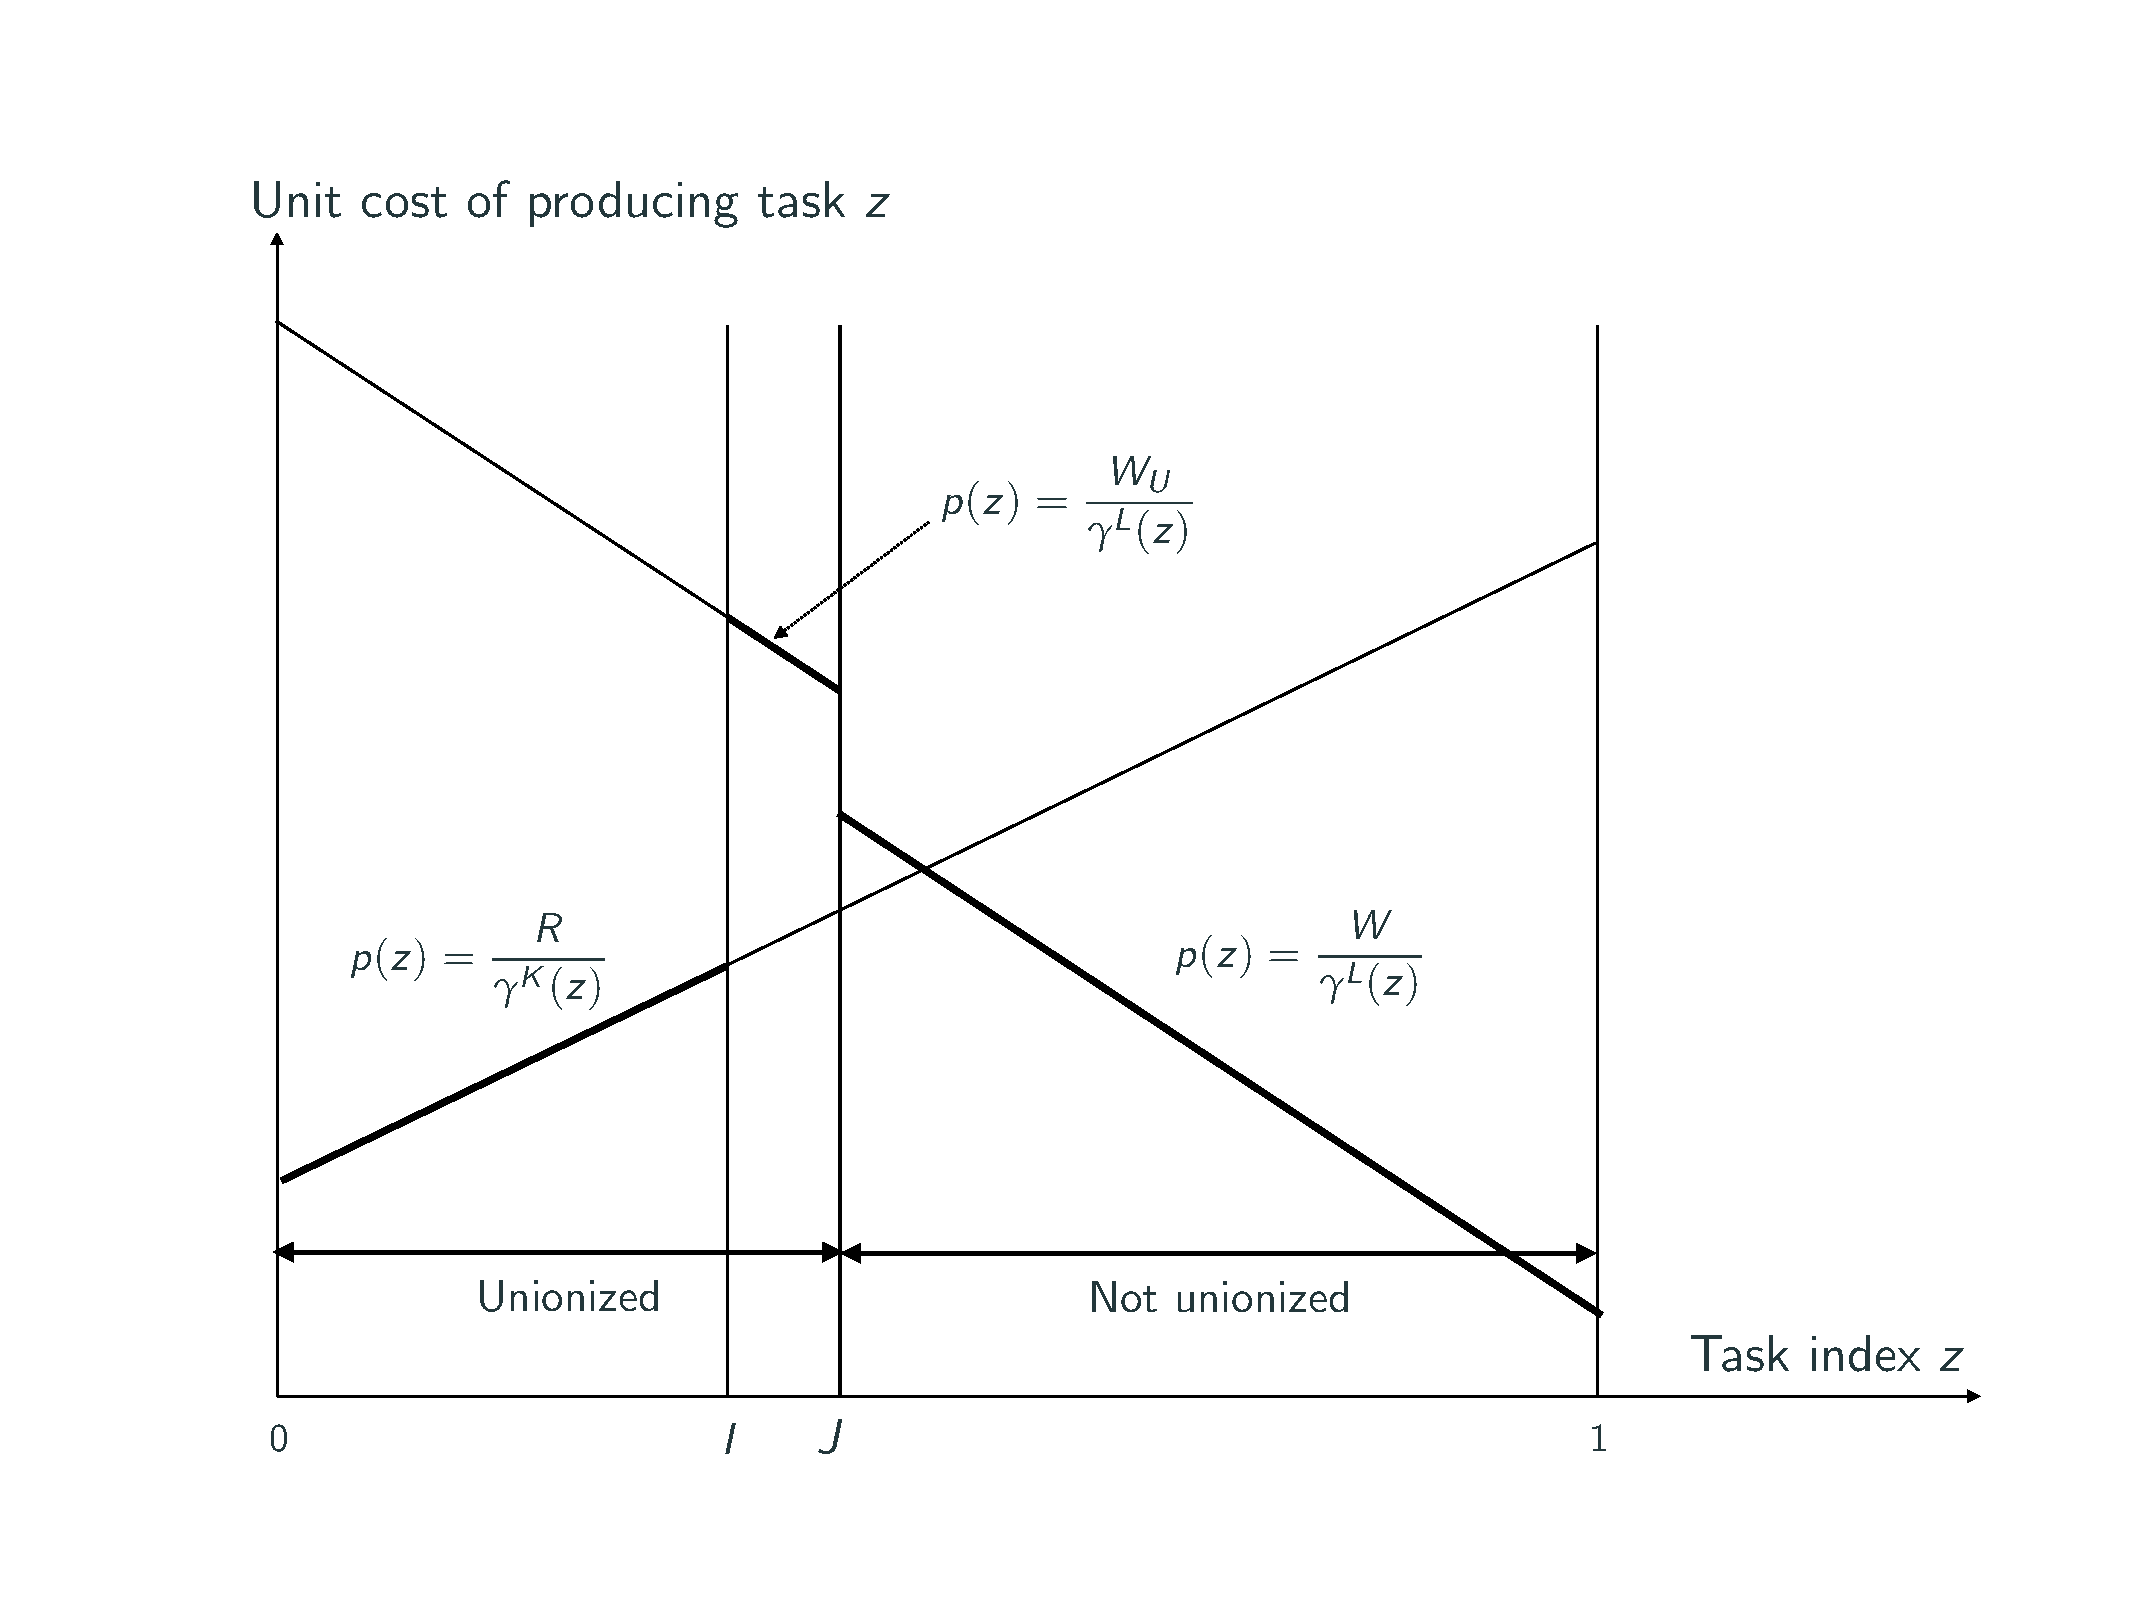
\includegraphics[width=0.6\paperwidth]{figures/figure2.pdf}
    \end{center}
\end{frame}

\frame{ \frametitle{Assumptions and equilibrium output}
\begin{itemize}
\item<1-> Tasks $0$ to $I$ are produced with $K$, and tasks $I$ to $1$ with $L$ \medskip
\item<1-> In union tasks $I$ to $J$, workers receive a union wage premium \medskip
\item<1-> Capital $K$ and labor $L$ are supplied inelastically \medskip
\item<1-> If tasks are combined Cobb-Douglas, equilibrium output can be written as:
\[
Y = \Psi_{H}(I) \left[ \frac{K}{I}\right]^{I} \left[ \frac{L_{U}}{J-I} \right]^{J-I} \left[ \frac{L-L_{U}}{1-J} \right]^{1-J} \nonumber
\]
with $L_{U}$ employment in union jobs and with
\[\Psi_{H}(I) \equiv \exp \left[ \int_{0}^{I} \ln(\gamma^{K}(z))dz + \int_{I}^{1} \ln(\gamma^{L}(z))dz \right] 
\]
\end{itemize}
}

\frame{ \frametitle{Automation of union jobs and labor demand}
\begin{itemize}
\item<1-> A union worker earns $W_{U} > W$ and wages equal marginal product \medskip
\item<1-> Automation of union jobs increases the gain in allocative efficiency such that automation of union jobs is less likely to decrease their marginal product of labor \medskip
\item<1-> Union workers displaced to non-union jobs experience stronger wage decreases \medskip
\item<1-> Impact on welfare is ambiguous because the direct allocative efficiency gain from automation opposes the loss in allocative efficiency from union workers moving to non-union jobs
\end{itemize}
}

\frame{ \frametitle{The impact of wage rents on allocative efficiency}
\noindent \begin{center}
	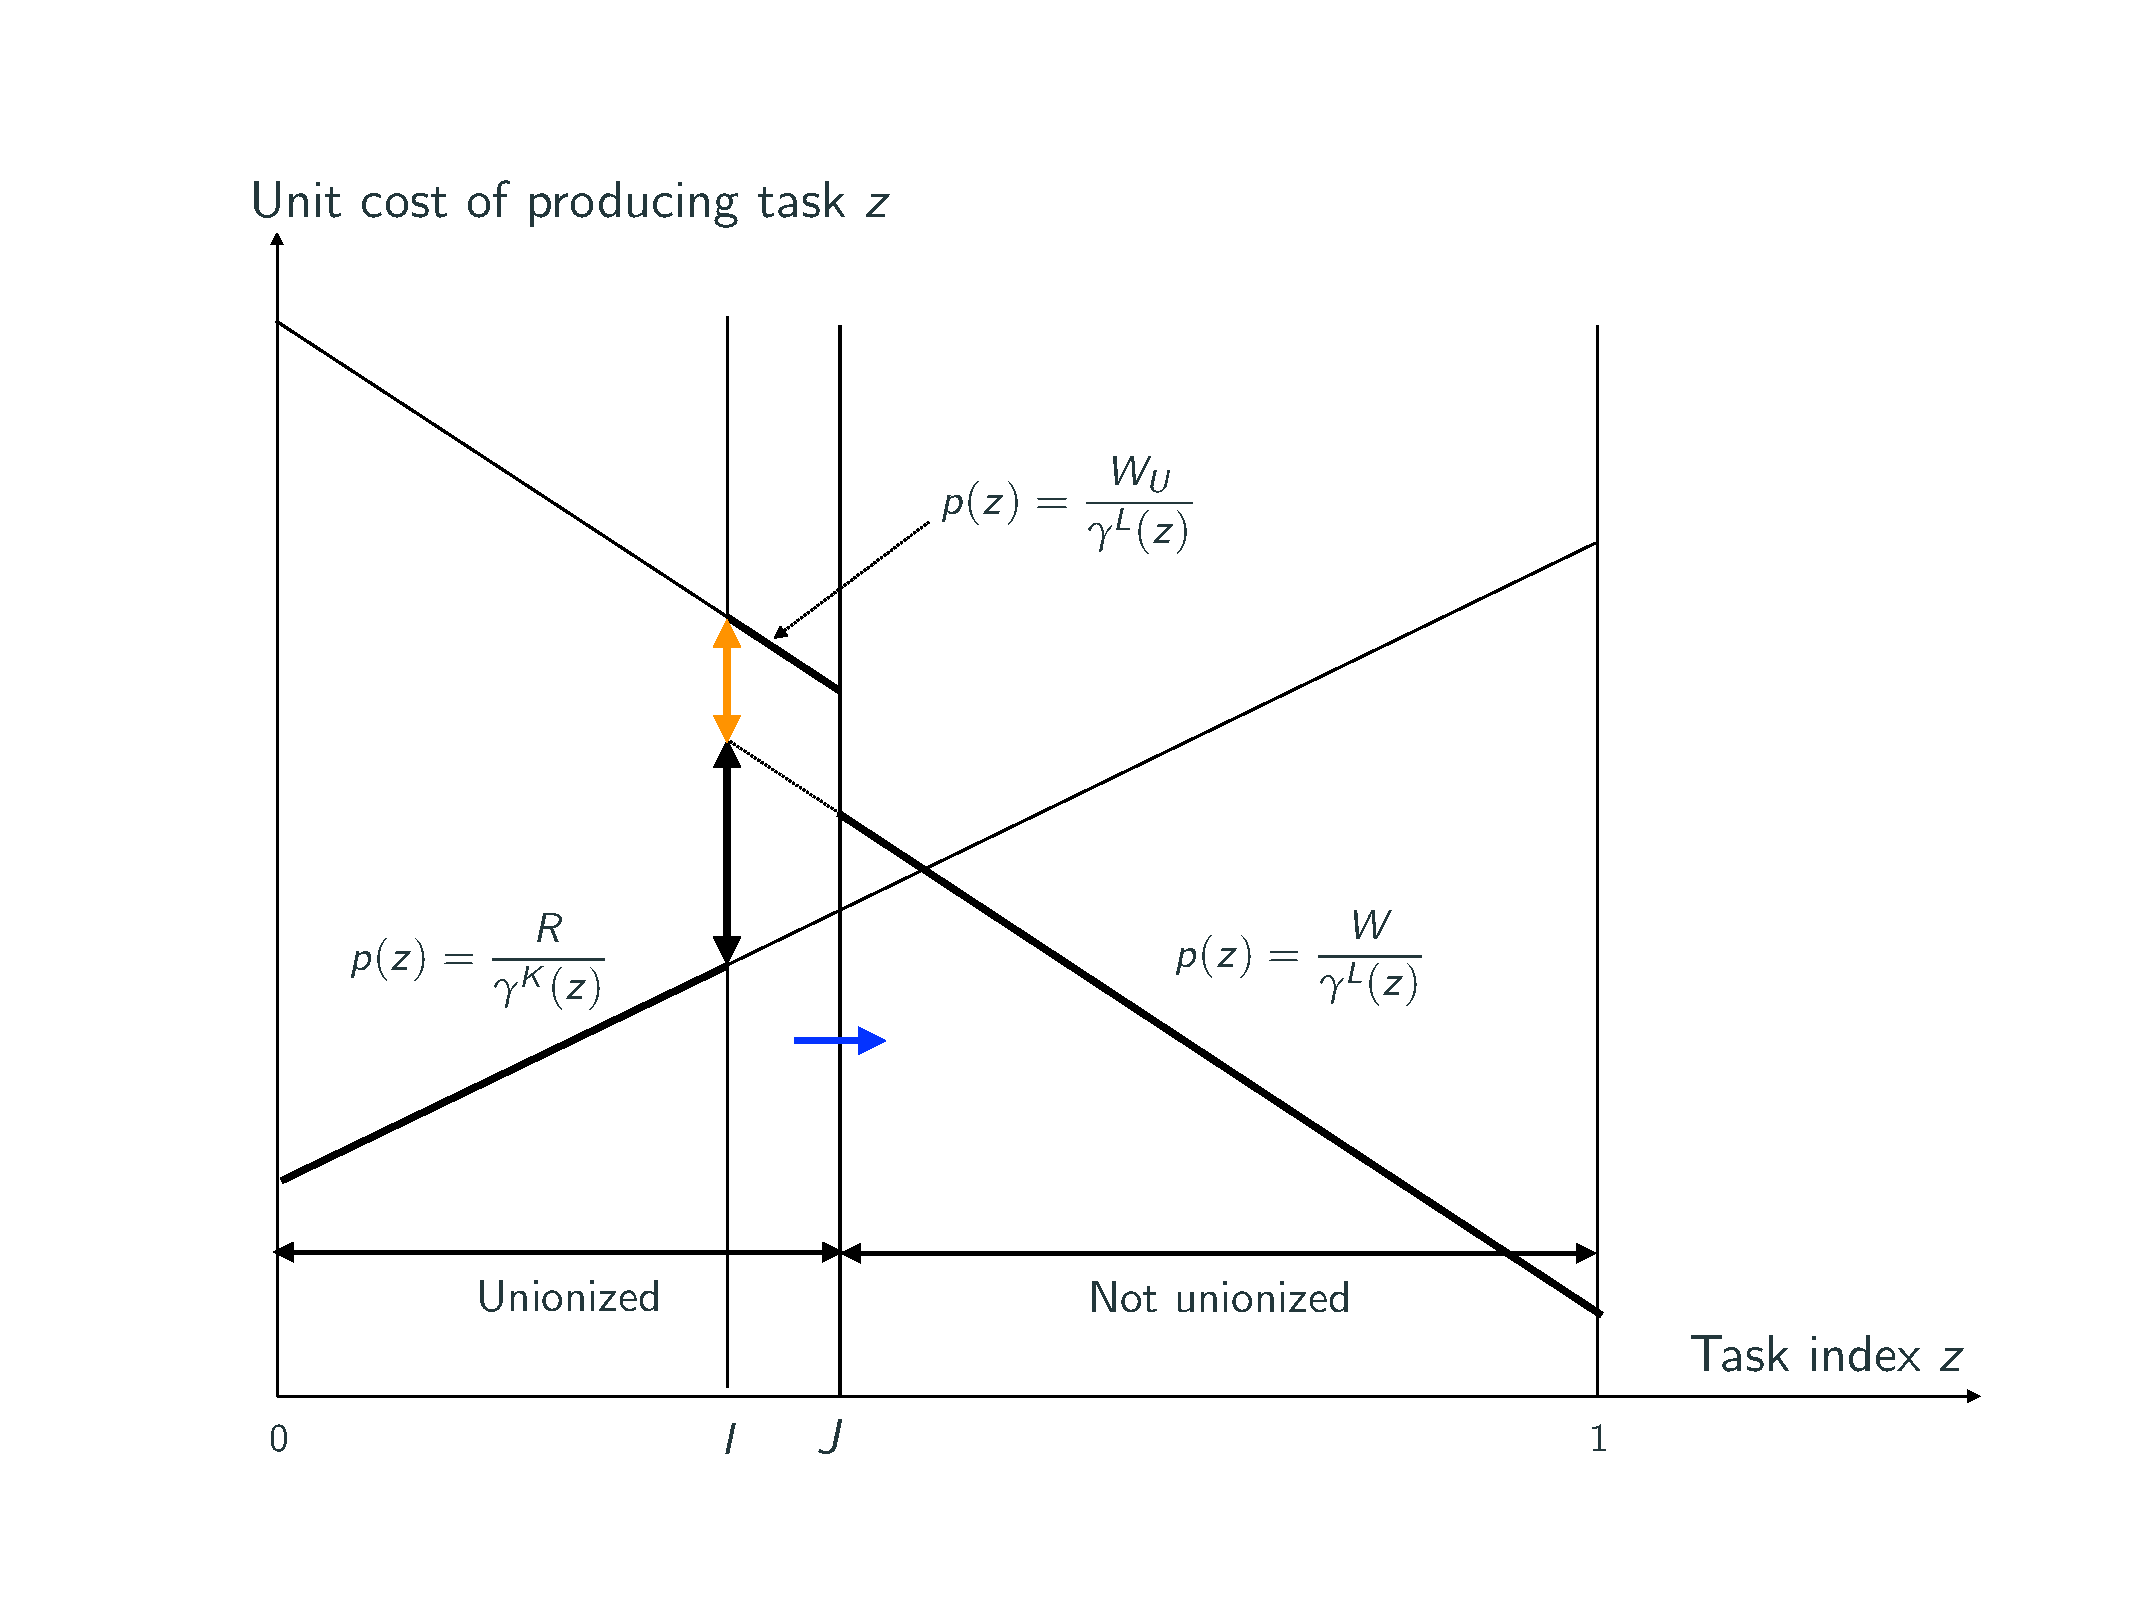
\includegraphics[width=0.6\paperwidth]{figures/figure3.pdf}
    \end{center}
}

\frame{ \frametitle{So-so automation of union jobs and allocative efficiency \hyperlink{distorted}{\beamerbutton{back}}}
\begin{itemize}
\item<1-> The change in $Y | K,L$ due to automation is given by:
\[
\frac{dY}{dI} = \frac{dY}{dI} |_{L_{U}} + W_{U} \frac{dL_{U}}{dI} +W\frac{d[L-L_{U}]}{dI}
\]
\item<1-> Using the expression for aggregate output above gives:
\begin{align*}
\frac{dY}{dI}  = & \underbrace{\left[ \ln \left( \frac{W}{\gamma^{L}(I)} \right) - \ln \left( \frac{R}{ \gamma^{K}(I)} \right) \right]Y}_{\text{Gain in allocative efficiency without union wage premium}} \\
& \underbrace{ \color{orange} \left[ \ln \left( \frac{W_{U}}{\gamma^{L}(I)} \right) - \ln \left( \frac{ W}{\gamma^{L}(I)} \right) \right]Y}_{\text{Extra gain in allocative efficiency}} \color{black} + \underbrace{\color{blue} [W_{U} - W] \frac{dL_{U}}{dI}}_{\text{Extra loss in allocative efficiency}}
\end{align*}
where the last term is negative given that $dL_{U}/dI <0$.
\end{itemize}
}

\end{document}
